\section{题目与摘要}
\begin{abstractbox}
\noindent\textbf{\heiti 摘\quad 要：}大语言模型训练成本高、周期长，损失尖峰、发散、过拟合等异常若不能及时发现和定位，会造成大量算力浪费。现有工具多停留在指标曲线展示层面，存在信号被噪声淹没、看得见却看不懂、日志本身不可靠、多运行比较视觉混乱等痛点。本文设计并实现了 TrainScope 系统：首先在字符级 GPT 训练中植入逐步、逐模块、逐注意力头的探针，完成 12 组真实训练（含学习率尖峰、标签污染、崩溃续训三类注入故障），得到 61,695 行多维日志；随后经过续训去重、计时污染修正、稳健 z 分数等清洗与特征工程，并用 PCA 和 t-SNE 对模块梯度与字符嵌入降维；在此基础上构建了一个包含 9 类联动视图、采用 focus+context 配色并支持自然语言操控的交互式仪表盘，以及“规划—监控—诊断—建议—报告”多智能体诊断工作流。实验表明：两次注入故障均在注入首步被检出，健康运行上没有误报，根因判别置信度分别为 99\% 与 98\%；学习率尖峰会造成中间层梯度坍缩式的不可逆损伤，而数据污染可以自行恢复；缺少预热会引发可恢复的注意力熵塌缩；字符嵌入中 96.2\% 的小写字母最近邻是其大写形式。系统代码与数据全部开源，可一键复现。

\vspace{0.5em}\noindent\textbf{\heiti 关键词：}训练监控；多维数据可视化；交互式可视分析；异常检测；多智能体；大语言模型
\end{abstractbox}

\section{引言与背景}

\subsection{业务需求分析}

大语言模型（LLM）训练是典型的高成本、长周期、强不确定性的工程活动。一次千亿参数级别的预训练往往需要数千张加速卡连续运行数周，单日算力成本可达数十万元。在这一场景中，训练过程本身就是需要被“观察”的对象：工程师需要随时回答“训练是否健康”“异常何时开始、源自哪里”“现在应当继续、回滚还是调整超参数”这三类问题。Meta 在 OPT-175B 的训练日志中记录了超过 35 次人工重启，多数源于损失尖峰与硬件故障\cite{r1}；BLOOM、PaLM 等报告也提到需要通过跳过数据批次、回滚检查点来化解损失尖峰\cite{r2,r3}。这些案例说明，训练监控并非“锦上添花”，而是直接决定算力浪费与项目成败的核心环节。

从可视化与交互的角度看，训练监控具有三个鲜明的数据特征：其一是\textbf{多尺度时序}，指标以“步”为单位高频产生（每秒数步至数十步），同时又需要在数千步尺度上观察趋势；其二是\textbf{高维结构化}，除标量损失外，每个模块的梯度、权重、更新比，每个注意力头的熵，都构成具有“层—模块—头”层级结构的高维张量序列；其三是\textbf{多运行对比}，超参数搜索与消融实验要求在同一视图中比较数十个运行。由此，本文抽象出以下业务需求：

\begin{itemize}
\item \textbf{R1 全局健康感知}：在一屏内掌握所有运行的健康等级、最优指标与异常数量；
\item \textbf{R2 异常的发现与定位}：自动发现损失尖峰、梯度爆炸、发散、停滞、过拟合等异常，并定位到具体步区间与具体模块；
\item \textbf{R3 根因解释与处置建议}：区分“学习率问题”“数据问题”“正则化问题”等不同根因，并给出可执行的建议（例如回滚到哪一步）；
\item \textbf{R4 内部表征洞察}：观察模型内部（注意力分布、嵌入空间）如何随训练演化；
\item \textbf{R5 低门槛交互}：支持以自然语言提问的方式驱动视图，降低排障门槛。
\end{itemize}

\subsection{核心痛点}

（1）\textbf{信息过载与信号淹没}。逐步损失天然带有小批量噪声，真实的异常信号往往被淹没在噪声中；而当指标扩展到逐模块、逐头之后，指标数量从个位数膨胀到数百个，人工逐一盯盘不可行。

（2）\textbf{“看见”不等于“看懂”}。损失曲线上的一个尖峰可能由学习率调度错误、上游数据损坏、数值溢出等完全不同的原因造成，处置方式截然不同：学习率问题需要回滚权重，而数据问题只需剔除对应分片。仅凭损失曲线无法区分二者，需要跨指标的联合取证。

（3）\textbf{日志本身不可靠}。真实训练日志存在断点续训造成的重复步、崩溃时的半行写入、评估开销污染的计时、发散后的 NaN/Inf 等“脏数据”。直接可视化原始日志会产生误导性的图形（例如重复步造成曲线回折，评估步造成周期性的伪吞吐下降）。

（4）\textbf{多运行比较的视觉混乱}。当 12 个以上运行叠加在同一坐标系，若为每个运行分配一种颜色，既超过人眼可区分的类别色上限，也使色觉障碍用户无法辨认。

\subsection{现有方案及其局限}

TensorBoard\cite{r4}是最早普及的训练可视化工具，以标量曲线、直方图和计算图为主，其局限在于：视图之间缺乏联动，没有跨运行的结构化比较，也不具备任何自动诊断能力。Weights \& Biases\cite{r5}与 MLflow 等实验管理平台提供了更完善的多运行比较与平行坐标图，但本质上仍是“指标仪表盘”：异常需要用户自己发现，告警规则需要用户手写阈值，并且模型内部的细粒度表征（如逐头注意力熵）需要用户自行埋点。学术界的可视分析工作，如 DeepTracker\cite{r6}对 CNN 训练过程的多层级可视化、Hohman 等人对深度学习可视分析的综述\cite{r7}，以及 BertViz\cite{r8}对 Transformer 注意力的可视化，都在某一方面做得比较深，但要么针对 CNN 而非 Transformer，要么只分析训练完成后的静态模型，很少把训练过程的动态监控和根因诊断放在同一个系统里。

近两年，基于大模型的智能体被用于数据分析，例如 LIDA\cite{r9}可以从数据自动生成可视化，Data Interpreter\cite{r21}等工作可以执行多步分析。不过把这类方法直接用于训练诊断，会碰到两个问题：一是大模型直接读原始曲线时容易编造数字；二是诊断结论缺乏可追溯的证据链。因此本文采用“统计检测器 + 取证工具 + 知识库评分”作为确定性的诊断主干，大模型只是可选的语言润色层，所有结论都以结构化证据为约束。

\subsection{本文工作}

针对上述需求与痛点，本文设计并实现了 TrainScope 系统，主要工作包括：（1）构建了一套带全量探针的 GPT 训练框架，通过 12 组真实训练运行（含 3 类真实注入故障）产生约 24.8 MB、61,695 行原始日志的多维监控数据集；（2）设计了面向训练日志的数据清洗与特征工程流程，并以 PCA 和 t-SNE 对高维梯度与嵌入数据进行规约；（3）实现了一个以 focus+context 为核心配色策略、包含 9 类联动视图的交互式仪表盘；（4）实现了 Planner–Monitor–Diagnostician–Advisor–Comparator–Reporter 多智能体诊断工作流与自然语言视图操控；（5）通过案例分析揭示了学习率、预热、裁剪、正则化对训练动力学的影响规律，并对异常检测的效果进行了事件级评估。

\section{数据预处理与特征工程}

\subsection{数据来源}

\textbf{训练语料}。本文采用 Karpathy 公开的 TinyShakespeare 语料\cite{r10}（莎士比亚剧作合集，1,115,394 个字符，65 个不同字符，SHA-256 前缀 86c4e6aa），按 9:1 切分为训练集与验证集。字符级语言建模任务计算量小、可在单卡上完成多组完整训练，同时保留了 Transformer 训练的全部典型动力学现象（预热、过拟合、注意力头特化等），适合作为大模型训练监控的“可控缩微实验场”。

\textbf{模型与训练配置}。模型为 Pre-LN 结构的 GPT 解码器\cite{r11}：基线 6 层、6 头、隐维 384、上下文 256，参数量 10.80M；扩容配置为 8 层、8 头、隐维 512，参数量 25.39M。优化器为 AdamW（$\beta$=(0.9,0.95)，权重衰减 0.1），学习率采用“线性预热 + 余弦衰减至 10\%”，bf16 混合精度，单卡 NVIDIA RTX 4090，每个运行 2,500 步（批量 64$\times$256，共 4,096 万字符，约 40.8 个 epoch 当量）。

\textbf{实验设计}。为了让监控数据覆盖健康、次优、故障三种状态，本文设计了表 1 所示的 12 组运行。其中 R09、R10、R11 为\textbf{真实注入的故障}：R09 在第 1200–1229 步将学习率临时放大 25 倍，模拟配置热更新错误；R10 在第 1800–1839 步将训练标签替换为均匀随机字符，模拟上游数据管道损坏；R11 在第 1400 步让进程真实退出，再从第 1000 步的检查点续训，从而在日志中产生真实的重复步与丢失记录。故障的起止位置已知，可以作为异常检测评估的真值。

\begin{table}[htbp]
\centering
\caption{实验运行设计}
\small
\begin{tabularx}{\linewidth}{XccccccX}
\toprule
\textbf{运行} & \textbf{峰值学习率} & \textbf{预热} & \textbf{裁剪} & \textbf{批量} & \textbf{dropout} & \textbf{规模} & \textbf{设计意图} \\
\midrule
R01\_baseline & 1e-3 & 200 & 1.0 & 64 & 0.2 & 6L/384 & 基线 \\
R02\_lr3e-4 & 3e-4 & 200 & 1.0 & 64 & 0.2 & 6L/384 & 学习率偏低 \\
R03\_lr3e-3 & 3e-3 & 200 & 1.0 & 64 & 0.2 & 6L/384 & 学习率偏高 \\
R04\_lr1e-2\_noclip & 1e-2 & 200 & 关 & 64 & 0.2 & 6L/384 & 过高学习率且不裁剪 \\
R05\_nowarmup & 3e-3 & 无 & 1.0 & 64 & 0.2 & 6L/384 & 去除预热 \\
R06\_noclip & 3e-3 & 200 & 关 & 64 & 0.2 & 6L/384 & 去除梯度裁剪 \\
R07\_bs16 & 1e-3 & 200 & 1.0 & 16 & 0.2 & 6L/384 & 小批量 \\
R08\_nodropout & 1e-3 & 200 & 1.0 & 64 & 0 & 6L/384 & 去除正则化 \\
R09\_fault\_lrspike & 1e-3 & 200 & 1.0 & 64 & 0.2 & 6L/384 & 注入：学习率$\times$25（1200–1229） \\
R10\_fault\_corrupt & 1e-3 & 200 & 1.0 & 64 & 0.2 & 6L/384 & 注入：标签污染（1800–1839） \\
R11\_crash\_resume & 1e-3 & 200 & 1.0 & 64 & 0.2 & 6L/384 & 注入：崩溃@1400，续训@1001 \\
R12\_large & 6e-4 & 200 & 1.0 & 64 & 0.2 & 8L/512 & 扩容 \\
\bottomrule
\end{tabularx}
\end{table}

\textbf{探针与采集频率}。训练脚本在不改变训练语义的前提下植入了四类探针（表 2）。模块级指标把参数归为 14 个可解释的模块组（embed、L\textit{i}.attn、L\textit{i}.mlp、head），梯度范数在裁剪之前计算，以便如实反映梯度尖峰。注意力熵和激活统计在一个固定的验证探针批次（8$\times$256 字符）上计算，这样不同步之间可以直接比较。更新比 $\|$$\Delta$W$\|$/$\|$W$\|$ 通过在优化器更新前后对参数做快照得到，它度量的是“这一步实际把权重改动了多少”，是判断学习率是否合适的关键指标\cite{r12}。

\begin{table}[htbp]
\centering
\caption{探针指标与采集频率}
\small
\begin{tabularx}{\linewidth}{XcXc}
\toprule
\textbf{文件} & \textbf{频率} & \textbf{字段} & \textbf{维度/步} \\
\midrule
scalars.jsonl & 每步 & loss, lr, grad\_norm(裁剪前), step\_time, tok/s, 显存峰值 & 8 \\
layers.jsonl & 每步 / 每10步 & 14 模块梯度范数；14 模块权重范数与更新比 & 14 / 42 \\
probes.jsonl & 每50步 & 层$\times$头注意力熵、逐层残差流 RMS 与最大激活 & 48（基线） \\
evals.jsonl & 每100步 & 训练/验证损失（各 20 批次均值） & 2 \\
embed\_tok.npy & 结束时 & 字符嵌入矩阵 & 65$\times$384 \\
\bottomrule
\end{tabularx}
\end{table}

\subsection{数据清洗流程}

原始日志直接来自训练进程，包含多种真实“脏数据”。本文按以下顺序进行清洗，每一步的统计结果写入质量报告（表 3），在仪表盘中也可以查看。

\textbf{（1）解析与类型规整}。JSON 不支持 NaN/Inf，训练脚本在损失非有限时以字符串形式写出，清洗时将其还原为 IEEE 浮点并标记；进程崩溃时可能留下半行 JSON，解析失败的行被计数后丢弃。

\textbf{（2）续训去重与丢失记录}。R11 在第 1400 步崩溃。由于日志采用带缓冲的追加写，且只在每 100 步时显式刷新，进程被强制终止时缓冲区中第 1373–1399 步的记录尚未落盘，直接丢失；而从第 1000 步检查点恢复后，第 1001–1372 步又被写入了第二次（共 372 个重复步）。由于续训后的轨迹才是最终模型真实经历的轨迹，本文按 step 去重并保留最后一次写入。图 2(a) 对比了被覆盖的崩溃前记录与保留的记录：两者损失水平接近但逐步取值不同，因为续训恢复了数据采样器的随机状态，而 dropout 的随机掩码无法逐位复现。如果不做去重直接按写入顺序画线，曲线会在第 1399 步“折返”到第 1001 步，读者很容易误以为训练出现了倒退。

\textbf{（3）缺口检测}。以 step 的连续整数序列为参照统计缺失步。R11 崩溃时丢失的 1373–1399 步在续训中被重新执行和记录，所以清洗后缺失步为 0；如果只看崩溃前的文件，这 27 步就是一个缺口。这说明“去重保留最后写入”的策略同时修复了丢失和重复两类问题。

\textbf{（4）计时污染修正}。训练脚本在第 50\textit{k} 步之后运行探针、在第 100\textit{k} 步之后运行评估，这部分耗时会被计入下一步的 step\_time，使吞吐曲线出现规律的周期性“下跌”（图 2(b)）。此外，第一步包含 CUDA 上下文初始化，耗时高出两个数量级。本文将 step\%50==1 的步、首步以及超过中位数 20 倍的步标记为 timing\_contaminated，在计算吞吐统计和检测吞吐下降时剔除，但在损失类分析中保留。以 R01 为例，正常步的中位耗时为 18.5 ms，被标记的污染步平均耗时 221.7 ms（约 12 倍）；剔除后平均吞吐由 86.7 万提升到 87.6 万 tokens/s。图 2(b) 中清洗后的曲线仍然每 10 步出现一个小凸起，这是更新比探针每 10 步对参数做快照造成的真实开销，并不是计时污染，因此保留。这也提示探针本身存在“观察者效应”，需要在频率和开销之间权衡。

\begin{figure}[htbp]
\centering
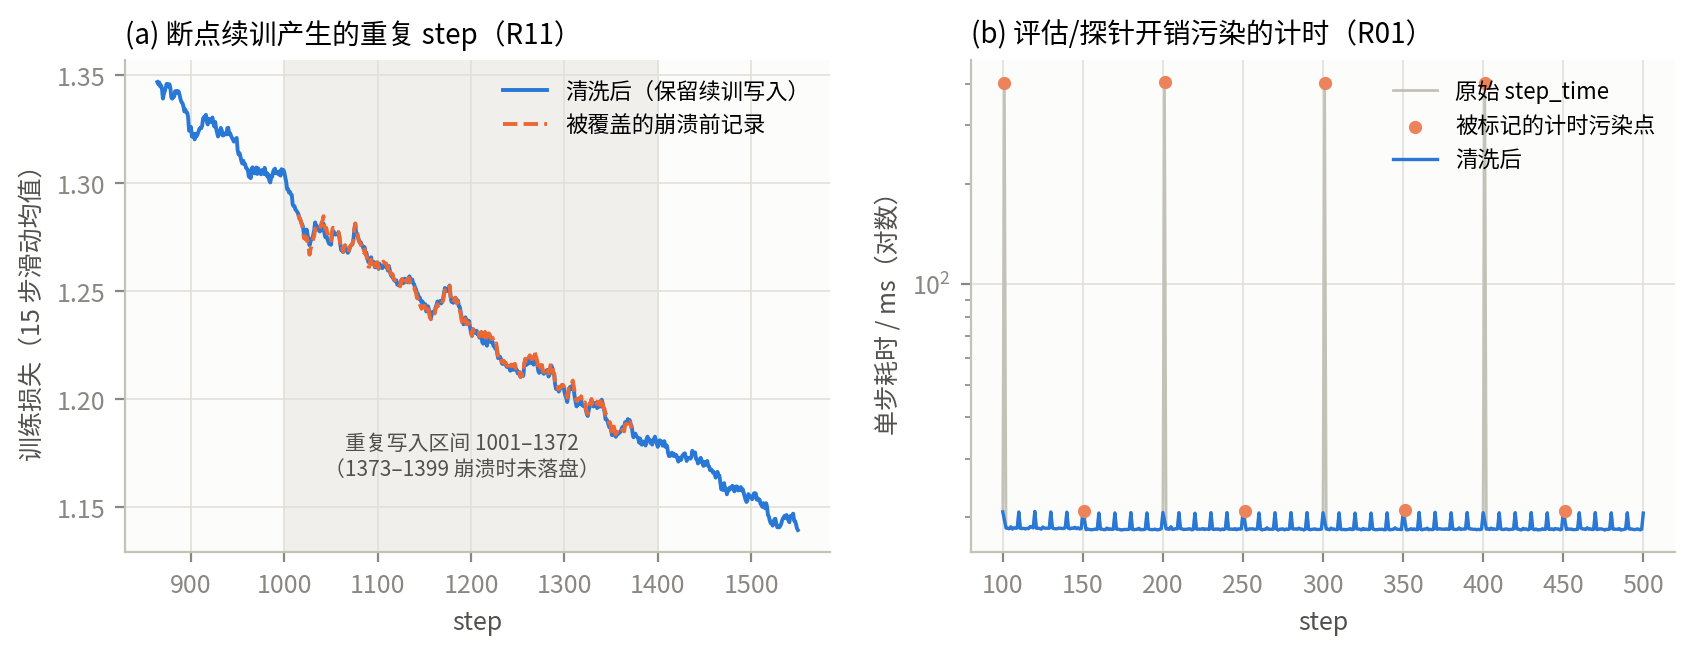
\includegraphics[width=\linewidth]{figures/fig_cleaning.png}
\caption{数据清洗示意：(a) 断点续训造成的重复步；(b) 评估开销对计时的污染}
\end{figure}

\textbf{（5）平滑}。为同时服务“趋势观察”与“尖峰检测”两种任务，本文计算两种平滑：指数滑动平均 EMA（$\alpha$=0.02）用于趋势展示；中心化滚动中位数（窗口 51）用于构造残差。中位数对尖峰不敏感，因此残差能够完整保留尖峰幅度。

\begin{table}[htbp]
\centering
\caption{数据质量报告（清洗统计）}
\small
\begin{tabularx}{\linewidth}{Xccccccc}
\toprule
\textbf{运行} & \textbf{原始行} & \textbf{坏行} & \textbf{重复步} & \textbf{缺失步} & \textbf{非有限损失} & \textbf{计时污染步} & \textbf{清洗后步数} \\
\midrule
R01–R10、R12（各） & 2,500 & 0 & 0 & 0 & 0 & 51 & 2,500 \\
R11\_crash\_resume & 2,872 & 0 & 372 & 0* & 0 & 51 & 2,500 \\
合计 & 30,372 & 0 & 372 & 0 & 0 & 612 & 30,000 \\
\bottomrule
\end{tabularx}
\end{table}

\noindent 注：表中“原始行”为 scalars.jsonl 的行数。* 崩溃前的日志文件缺少第 1373–1399 步（共 27 步），续训后补齐。

值得一提的是，R04（学习率 1e-2、不裁剪）虽然梯度范数峰值达到 2,252，却没有出现 NaN。原因是 bf16 的指数范围与 fp32 相同，而且 AdamW 的更新幅度会被二阶矩归一化，单步更新不会随梯度一起无限放大。这一点说明，“没有 NaN”不能当作训练健康的依据，需要另外设计停滞和退化类检测器（见 4.4 节）。

\subsection{特征工程}

在清洗后的逐步数据上，本文构造了以下特征：

\begin{itemize}
\item \textbf{损失残差} $r_t=\ell_t-\operatorname{median}(\ell_{t-25:t+25})$，刻画偏离局部趋势的程度；
\item \textbf{滚动波动率}：一阶差分在 51 步窗口内的标准差，衡量优化噪声水平；
\item \textbf{稳健 z 分数}：$z_t=(x_t-\mathrm{med})/(1.4826\cdot\mathrm{MAD})$，其中 med 与 MAD 在 101 步窗口内计算。相比均值—标准差 z 分数，它不会被尖峰本身“拉高基线”而自我掩盖，1.4826 为正态分布下 MAD 到标准差的一致性因子；
\item \textbf{对数梯度范数}：梯度范数跨越 4 个数量级（10\textsuperscript{$-$2}–10\textsuperscript{3}），取对数后分布接近对称；
\item \textbf{更新比跃升}：各模块更新比的最大值相对自身前序 200 步中位数的倍数；
\item \textbf{运行级摘要}：最优/最终验证损失、最优步、泛化差（最终验证$-$训练损失）、过拟合回升量（最终验证$-$最优验证）、梯度范数 P99、吞吐中位数等 20 个字段，用于平行坐标与总览表。
\end{itemize}

\subsection{维度规约}

\textbf{训练状态轨迹（PCA）}。对每个运行，以 50 步为窗口，计算 14 个模块梯度范数的对数均值，得到一个 14 维的“训练状态向量”。11 个 6 层运行（R12 为 8 层，模块集合不同，不纳入同一特征空间）的窗口向量合并后按列标准化，再用 SVD 求主成分。这样每个运行在训练过程中的状态变化就成为二维平面上的一条轨迹，不同运行的“优化路径”可以直接比较。PCA 是线性的、可逆的，载荷可以解释，适合需要说明“轴代表什么”的监控场景。

\textbf{嵌入空间（t-SNE）}。对基线模型最终的 65$\times$384 字符嵌入矩阵，本文用 numpy 实现了精确 t-SNE\cite{r13}（二分搜索匹配困惑度 10，早期夸大系数 12，动量 0.5$\rightarrow$0.8，自适应增益，1000 次迭代），同时给出 PCA 投影作对照。t-SNE 更擅长保留局部邻域，可以揭示模型学到的“字符类别”结构。所有降维算法都只依赖 numpy，没有引入 scikit-learn，因此在离线或受限的训练集群上也能直接部署。

\subsection{探索性数据分析（EDA）}

在设计检测器和视图之前，本文先对清洗后的数据做了探索性分析（图 3）。

\begin{figure}[htbp]
\centering
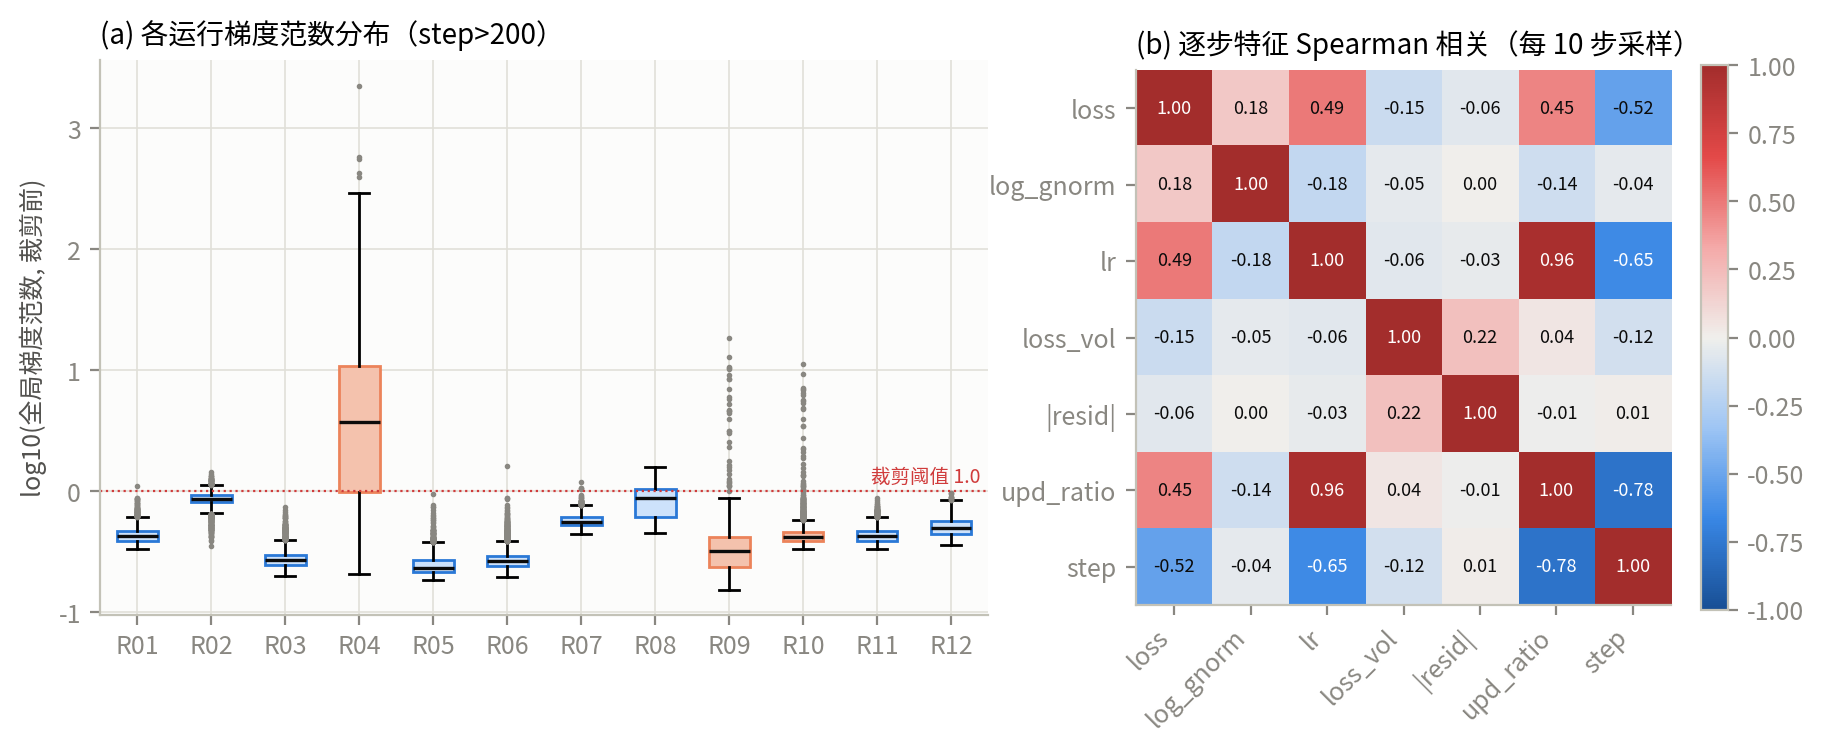
\includegraphics[width=\linewidth]{figures/fig_eda.png}
\caption{探索性分析：(a) 各运行裁剪前全局梯度范数分布（对数，step>200，橙色为异常运行）；(b) 逐步特征的 Spearman 秩相关矩阵}
\end{figure}

\textbf{（1）梯度范数分布}。健康运行的梯度范数集中在 0.2–1.0（对数 $-$0.7–0），四分位距都很窄。R04 的中位数为 2.96，69.8\% 的步超过裁剪阈值 1.0，上须延伸到 10\textsuperscript{2.5}，属于“慢性”梯度异常。R09 与 R10 的箱体本身正常，但有大量离群点，属于“急性”异常。两类异常的分布形态不同，说明单一阈值无法兼顾：急性异常适合用相对于局部基线的稳健 z 分数检测，慢性异常则需要对运行级统计量（P99、停滞）做判断。另一个有意思的现象是，学习率最低的 R02 反而有最高的健康梯度范数（中位约 0.85）。较小的学习率让优化停留在曲率较高的区域，这与“稳定性边缘”（edge of stability）的经验观察一致\cite{r16}。

\textbf{（2）特征相关性}。更新比与学习率的秩相关高达 0.96，说明对 Adam 类优化器而言，更新比几乎完全由学习率调度决定，所以检测器必须看更新比相对于自身基线的“跃升”，而不能用绝对阈值。早期版本的检测器使用 1e-2 的绝对阈值，在 R03 等高学习率但完全健康的运行上产生了大量误报，这正是在 EDA 之后被修正的。对数梯度范数与损失的相关只有 0.18，说明梯度大小本身不是可靠的健康信号。损失残差的绝对值与其他所有特征几乎不相关（|$\rho$|$\le$0.22），说明尖峰是独立的突发事件，无法通过回归趋势来预测，这为采用“事件检测”而不是“趋势回归”的设计提供了依据。

\section{可视化设计与系统实现}

\subsection{系统架构}

TrainScope 采用四层架构（图 1）。采集层是带探针的训练进程，以 JSONL 追加写入日志，对训练吞吐的影响可以控制。预处理与特征层负责清洗、特征计算和降维，输出结构化表格。智能诊断层由多智能体工作流组成，产出异常事件、根因、建议和执行轨迹。可视化交互层是一个纯静态的单页应用（ECharts 5.5），数据以 JSON 形式内嵌，不需要服务器，直接用浏览器打开即可使用，便于作为训练产物归档和分享。

\begin{figure}[htbp]
\centering
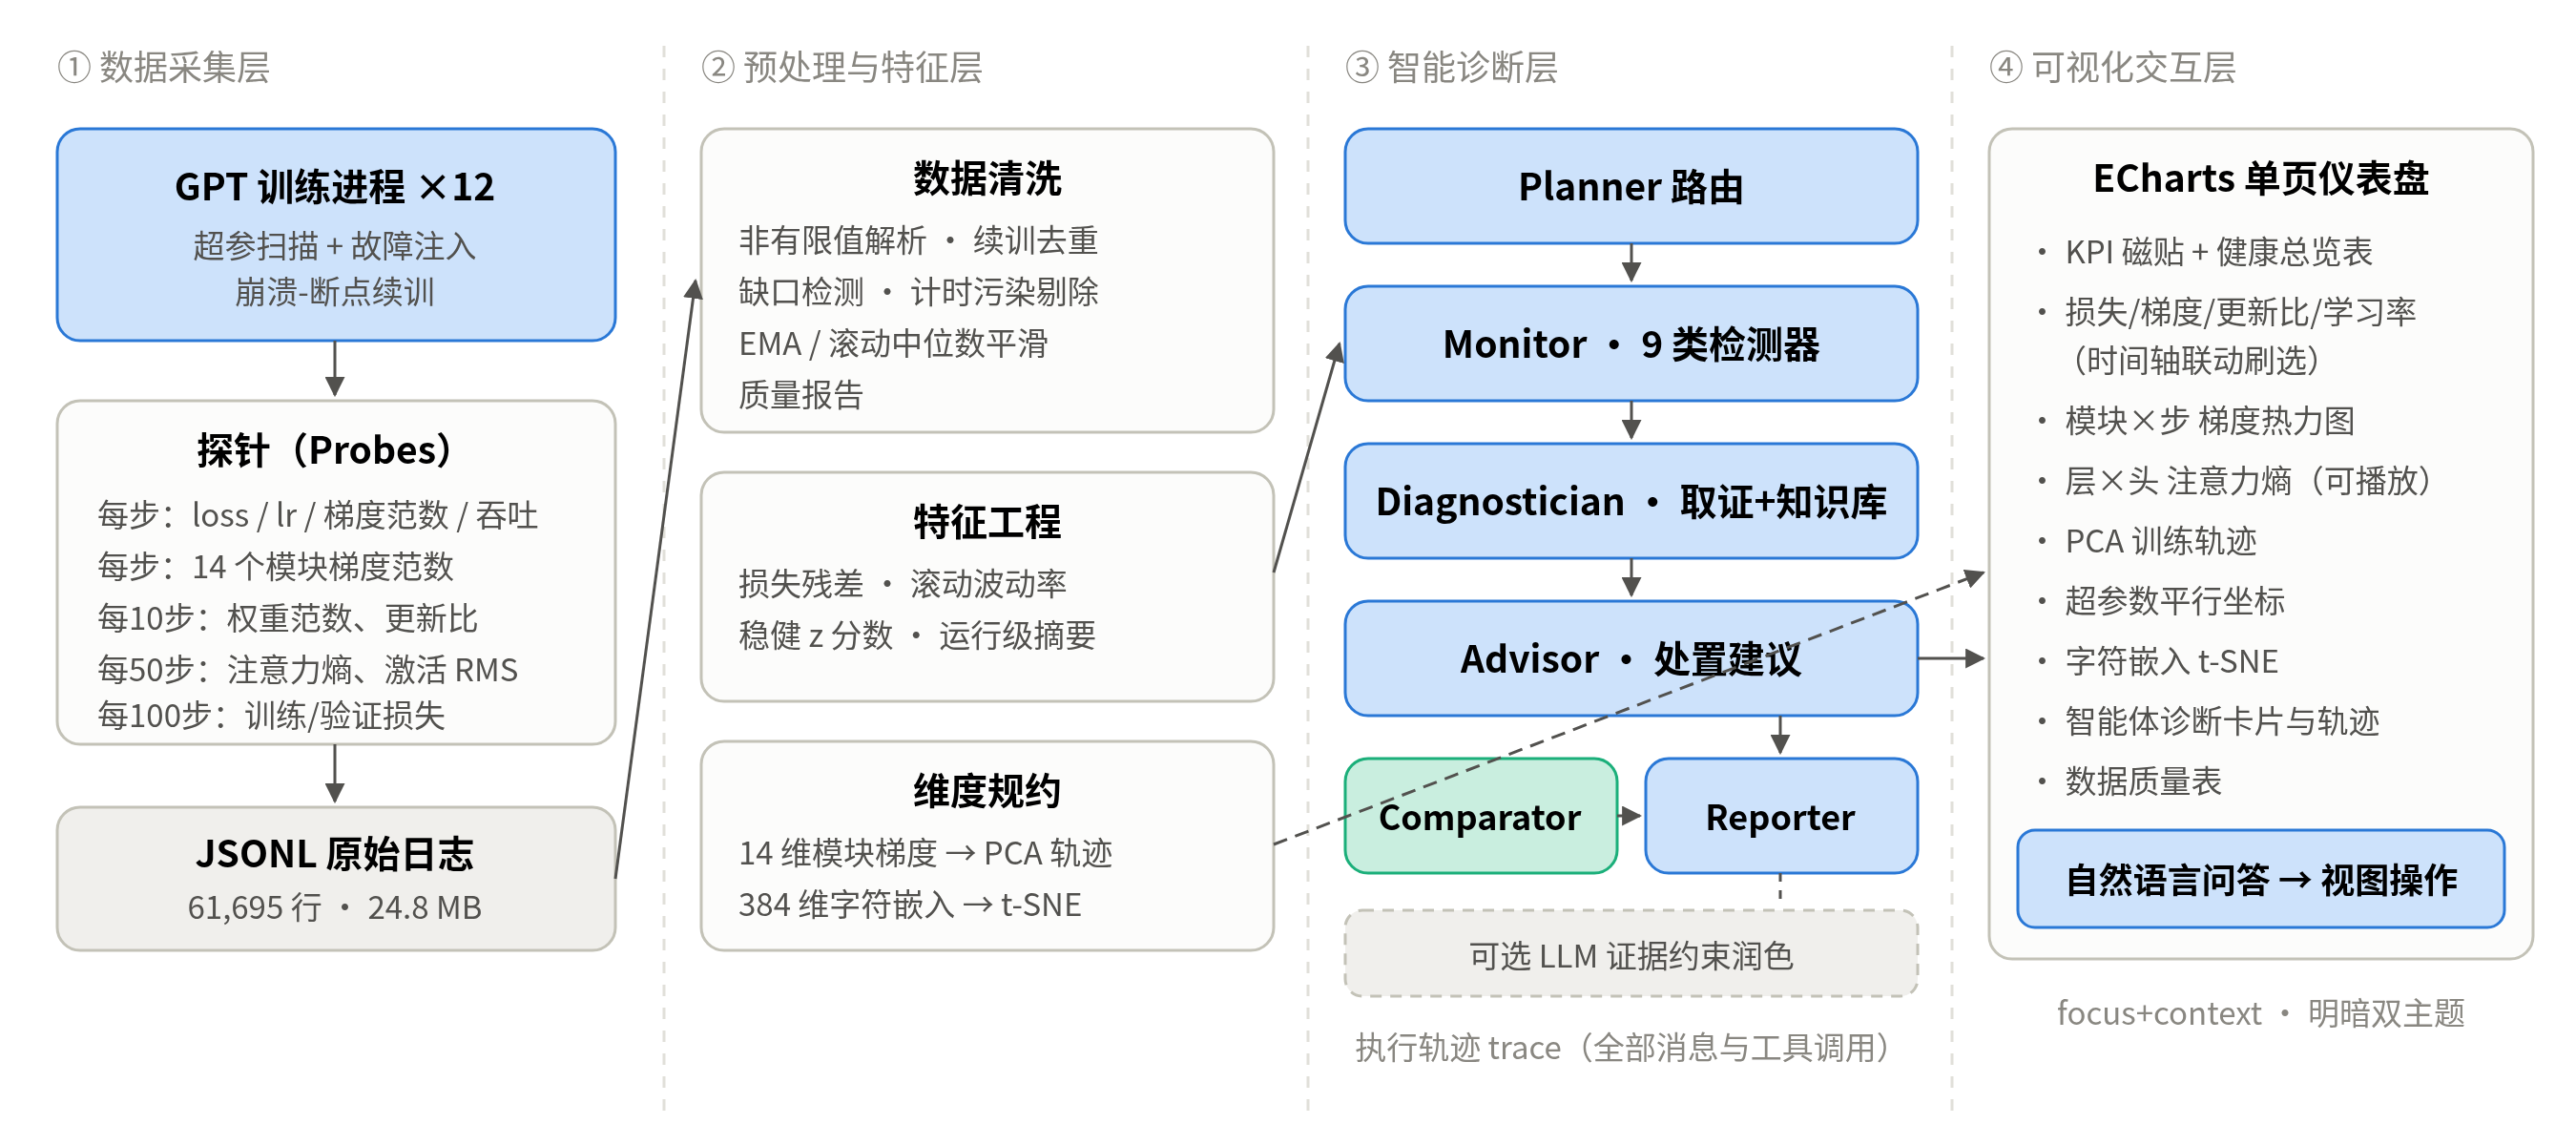
\includegraphics[width=\linewidth]{figures/arch.png}
\caption{TrainScope 系统架构图}
\end{figure}

\subsection{图表选型逻辑}

本文的选型原则是\textbf{由数据的“任务”决定图表形式，而不是由美观决定}。按 Munzner 的“What–Why–How”框架\cite{r14}，每个视图先明确数据抽象（数据是什么）与任务抽象（用户要做什么），再选择视觉编码。表 4 汇总了九个核心视图的选型依据。

\begin{table}[htbp]
\centering
\caption{视图选型依据}
\small
\begin{tabularx}{\linewidth}{XXXX}
\toprule
\textbf{视图} & \textbf{数据抽象} & \textbf{任务} & \textbf{编码选择与理由} \\
\midrule
损失曲线 & 多运行时间序列 & 趋势、比较、异常定位 & 折线（位置编码最精确）；逐步 EMA 实线与验证虚线分形；异常用半透明色带 \\
梯度范数 & 跨 4 个数量级的时间序列 & 发现尖峰 & 对数 y 轴，避免尖峰把正常区间压扁；裁剪阈值参考线 \\
更新比 / 学习率 & 时间序列 & 关联验证 & 各自独立坐标的小图（拒绝双 y 轴），共享 x 轴并联动 \\
模块$\times$步热力图 & 二维矩阵（14$\times$250） & 定位异常模块 & 单色顺序色板（浅$\rightarrow$深蓝），对数色标；行按网络深度排序 \\
注意力熵 & 层$\times$头矩阵序列 & 观察特化与塌缩 & 带数值标签的热力图 + 时间滑块动画 \\
PCA 轨迹 & 14 维向量序列 & 比较优化路径 & 连线散点图（connected scatter），起终点用不同形状 \\
平行坐标 & 8 维运行属性 & 超参数—结果关联 & 平行坐标 + 轴上刷选；学习率轴对数化 \\
嵌入投影 & 65 个 384 维点 & 发现类别结构 & 散点 + 字符直接标注，形状作为颜色之外的冗余编码 \\
总览表 / KPI & 运行级摘要 & 排序、查值 & 表格（精确查值）+ 状态徽章（图标+文字+颜色） \\
\bottomrule
\end{tabularx}
\end{table}

\textbf{配色策略}。12 个运行远超类别色的可辨上限。本文采用经过验证的类别色板，并且只使用其前三个槽位（蓝、橙、青），这三种颜色在全色觉、红绿色盲和蓝黄色盲模拟下两两之间的 OKLab 色差都大于 8。由此形成 \textbf{focus+context} 策略：焦点运行固定为蓝色，最多两个对比运行依次为橙、青，其余运行一律作为浅灰色背景。“颜色跟随实体而非排名”：切换焦点时颜色随运行身份重新分配，但同一时刻同一运行的颜色在所有视图中一致。序列数据（热力图）只使用单一蓝色的明$\rightarrow$暗色阶，发散数据（相关矩阵）使用蓝—灰—红色板，中点为中性灰。状态色（良好/关注/警告/危险）与类别色互相隔离，并且总是和图标（\checkmark{} ! $\blacktriangle$ $\times$）及文字一起出现，避免只靠颜色传递含义。仪表盘为暗色模式单独选取了一套色阶，而不是简单反色。

\textbf{拒绝双 y 轴}。损失与学习率、梯度范数与更新比的量纲完全不同。双 y 轴图会诱导读者比较两条曲线的“交叉点”，而交叉点的位置完全取决于两个坐标轴的任意缩放，没有意义。本文改用共享 x 轴的多个小图，通过联动缩放和十字准线建立对应关系。

\subsection{交互设计方案}

交互设计遵循 Shneiderman 的“先概览，再缩放过滤，按需查看细节”信息检索箴言\cite{r15}，并实现了以下交互：

\begin{enumerate}
\item \textbf{概览}：页面顶部的 KPI 磁贴与右侧“运行健康总览表”给出全局状态；表格支持按任意列排序，点击某行即将其设为焦点运行，全部视图同步刷新。
\item \textbf{联动缩放（Brushing \& Linking）}：损失、梯度、更新比、学习率四个时间视图共享同一步区间。在任一视图中框选、滚轮缩放或拖动滑块，其余三个视图以及模块热力图都会同步到相同区间，实现“一处选择，多处高亮”。
\item \textbf{跨视图钻取}：点击损失曲线上的某一步，注意力熵视图会跳到最近的探针时刻；点击 PCA 轨迹上的某个点，会把该运行设为焦点，同时把时间视图缩放到该点附近；点击诊断卡片中的异常事件，时间视图缩放到事件区间（前后各留 200 步上下文），注意力视图定位到事件起点。
\item \textbf{时间动画}：注意力熵视图提供播放按钮和滑块，可以按 50 步间隔播放全部探针时刻，直观看到注意力头从均匀分布逐渐特化的过程。
\item \textbf{对比选择}：通过“对比运行”标签最多添加两个对比运行（第三个加入时最早的自动移出，保证颜色不超过三种），也可以关闭“其余运行作灰色背景”，进一步降低视觉噪声。
\item \textbf{细节按需}：所有图元都带悬停提示，时间序列用十字准线显示同一步所有可见运行的数值，热力图显示模块名、步区间和原始数值（不是对数值），方便精确查值。
\item \textbf{自然语言交互}：顶部问答框通过轻量级意图识别，把自然语言问题映射为视图操作（表 5），回答文本与视图变化同时出现，形成“问—看—答”闭环。
\item \textbf{状态可分享}：焦点运行、对比运行、缩放区间、主题和问题都可以写进 URL 参数，复制链接即可把当前的分析现场交给同事。
\end{enumerate}

\begin{table}[htbp]
\centering
\caption{自然语言意图与视图操作映射}
\small
\begin{tabularx}{\linewidth}{XXXX}
\toprule
\textbf{示例问题} & \textbf{识别意图} & \textbf{视图操作} & \textbf{回答内容} \\
\midrule
哪个运行最好？ & 排名查询 & 聚焦最优运行 & 前三名及其最优验证损失 \\
R09 为什么出问题？ & 单运行诊断 & 聚焦、缩放到首个异常、滚动到诊断卡片 & 事件、根因与置信度、建议 \\
比较 R01 和 R12 & 对比 & 设为焦点 + 对比 & 关键指标对照与胜者 \\
看 1150 到 1350 步 & 时间过滤 & 全部时间视图联动缩放 & 确认区间 \\
哪些过拟合了？ & 属性筛选 & 回升量最大的三个运行 & 各运行最优步与回升量 \\
\bottomrule
\end{tabularx}
\end{table}

\subsection{AI 智能体工作流}

诊断层采用编排者—工作者（Orchestrator–Worker）式的多智能体结构，共六个角色，职责互不重叠，通过结构化消息协作：

\begin{itemize}
\item \textbf{Planner（规划者）}：读取运行级摘要，为每个运行生成执行路线。例如已发散的运行会走“发散诊断”分支，而不是常规的尖峰检测。
\item \textbf{Monitor（监控者）}：调用 9 类统计检测器（表 6），把逐步信号转换成带证据的“事件”（起止步、严重度、证据字典）。相邻异常步按间隔合并，避免一次尖峰触发几十条告警。
\item \textbf{Diagnostician（诊断者）}：针对每个事件调用取证工具 \texttt{metrics.window}，提取事件窗口和前序对照窗口的学习率比、损失峰值、梯度放大倍数、更新比变化、验证损失变化、各模块放大倍数的离散度等证据，然后在根因知识库中为每个候选根因累加规则得分，再用 softmax 转换为置信度。
\item \textbf{Advisor（建议者）}：把最可能的根因映射成带参数的可执行建议，例如“从 $\le$1200 步的检查点回滚”“隔离第 1800–1840 步的数据分片”。
\item \textbf{Comparator（比较者）}：跨运行排序，并分析学习率敏感性。
\item \textbf{Reporter（报告者）}：汇总为中文诊断报告。检测到 \texttt{ANTHROPIC\_API\_KEY} 时，把结构化证据交给大模型（默认 claude-opus-5-5）改写成自然语言简报，并在提示词中要求“不得引入证据之外的数字”；否则使用确定性模板。本文全部实验都在离线模板模式下完成，以保证可复现。
\end{itemize}

\begin{table}[htbp]
\centering
\caption{Monitor 的异常检测器}
\small
\begin{tabularx}{\linewidth}{XXc}
\toprule
\textbf{检测器} & \textbf{判据} & \textbf{严重度} \\
\midrule
发散 divergence & 出现非有限损失，或 300 步后平滑损失 > 4.0（接近 ln65） & 严重 \\
损失尖峰 loss\_spike & 损失相对滚动中位数的稳健 z > 8，合并间隔 15 步 & 中/高 \\
梯度爆炸 grad\_explosion & log 梯度范数稳健 z > 6，且 > 5$\times$滚动中位数，合并间隔 100 步 & 高 \\
更新比跃升 large\_update & 模块最大更新比 > 4$\times$前序 200 步中位数，且 > 0.004 & 高 \\
收敛停滞 stagnation & 1000 步后平滑训练损失始终 > 2.0 & 高 \\
注意力塌缩 attention\_collapse & 全部头的平均注意力熵 < 0.5 nats & 高 \\
持续退化 regression & 验证损失高于历史最优 0.3 以上，且泛化差 < 0.15（训练损失同样恶化） & 严重 \\
过拟合 overfitting & 验证损失较历史最优回升 > 0.04，且最终泛化差 > 0.15 & 中 \\
吞吐下降 throughput\_drop & 剔除计时污染后，25 步滚动中位吞吐 < 0.7$\times$全程中位数 & 低 \\
\bottomrule
\end{tabularx}
\end{table}

知识库的核心思想是\textbf{区分性证据}。以“学习率异常”和“数据污染”这两种都会造成损失尖峰的根因为例，知识库中有三条关键规则：(a) 若事件窗口的学习率是前序窗口的 3 倍以上，则支持学习率根因（+3）；(b) 若损失峰值超过均匀分布的交叉熵 ln65$\approx$4.17，且学习率没有变化，则支持数据污染（+3）——训练良好的模型比随机猜测还差，只可能是目标与输入不一致：模型对“正确”字符很自信，而标签被随机替换，损失可以远高于 ln\textit{V}；(c) 若训练损失飙升（峰值比前序均值高 1.0 以上），而验证损失几乎不变，说明权重并未受损，异常只存在于输入数据中，支持数据污染（+2）；反之若验证损失同步上升，则支持学习率根因（+1）。规则 (c) 实际上把“验证集”当成了一个不受污染的对照组。代码片段如下：

\begin{Verbatim}[fontsize=\small,frame=single,breaklines,breakanywhere]
add("学习率过高/学习率调度异常", dyn and lr_r > 3, 3.0, f"事件窗口学习率为前序窗口的 {lr_r:.1f} 倍")
add("数据管道污染（标签/样本异常）", shock and loss_max > LN_V - 0.6 and lr_r < 1.5, 3.0,
    f"损失峰值 {loss_max:.2f} 超过均匀猜测熵 ln65={LN_V:.2f}，而学习率未变")
add("数据管道污染（标签/样本异常）", shock and vjump < 0.1 and lr_r < 1.5 and loss_max > loss_pre + 1.0, 2.0,
    f"训练损失飙升但验证损失仅变化 {vjump:+.2f}，异常来自输入数据而非权重")
...
H["其他/未知原因"] = [1.0, ["基准假设"]]   # 避免单一假设时置信度虚高为 100%
ks = list(H); sc = np.array([H[k][0] for k in ks]); conf = np.exp(sc) / np.exp(sc).sum()
\end{Verbatim}

每条规则命中时都会记录一条人类可读的“依据”，并随置信度一起展示在诊断卡片上。所有智能体之间的消息和工具调用都写入执行轨迹（trace），轨迹中包含智能体名称、消息类型、所属运行、耗时和内容，仪表盘的“多智能体工作流与执行轨迹”面板会以节点图和日志两种形式回放（节点大小表示消息数量），这样每一条诊断结论都可以追溯到具体的取证数据。

\subsection{实现细节与开源}

系统核心代码约 1,250 行 Python 与 420 行 HTML/JavaScript，依赖只有 PyTorch、numpy、pandas、scipy 和 matplotlib。\texttt{run\_all.sh} 可以一键复现“训练 $\rightarrow$ 预处理 $\rightarrow$ 诊断 $\rightarrow$ 出图 $\rightarrow$ 仪表盘”的全流程：在单卡 RTX 4090 上，12 组训练约需 30 分钟，其余分析步骤不到 1 分钟。仪表盘是纯静态文件（HTML + 2.1 MB 数据 + ECharts），双击即可离线打开，适合作为训练产物随检查点一起归档。全部源码、原始日志、处理结果和论文源文件都以 MIT 协议开源在 GitHub 仓库 \url{https://github.com/RowanDVega/computer-visualization-final}，目录结构与使用方法见仓库 README；克隆后直接用浏览器打开 \texttt{web/index.html} 即可体验交互式 Demo。

\section{案例分析与结果讨论}

\subsection{全局概览：12 个运行的健康画像}

图 4 是仪表盘的首屏，焦点运行为 R09（学习率尖峰），对比运行为基线 R01，其余运行作为灰色背景。KPI 磁贴显示 R09 处于“$\times$ 危险”状态，共 4 个异常事件，最优验证损失 1.4753 出现在第 1100 步。损失曲线上，第 1200 步之后蓝色曲线陡然抬升，并且在剩余 1300 步中始终没有回到灰色背景运行所在的区域，红色色带标出了“持续退化”区间。更新比和学习率小图在同一位置出现了尖峰，与损失曲线对齐。右侧总览表按最优验证损失升序排列，四档健康徽章（\checkmark{} 健康、! 关注、$\blacktriangle$ 警告、$\times$ 危险）用图标、文字和颜色三重编码。表 7 汇总了全部运行的结果。

\begin{figure}[htbp]
\centering
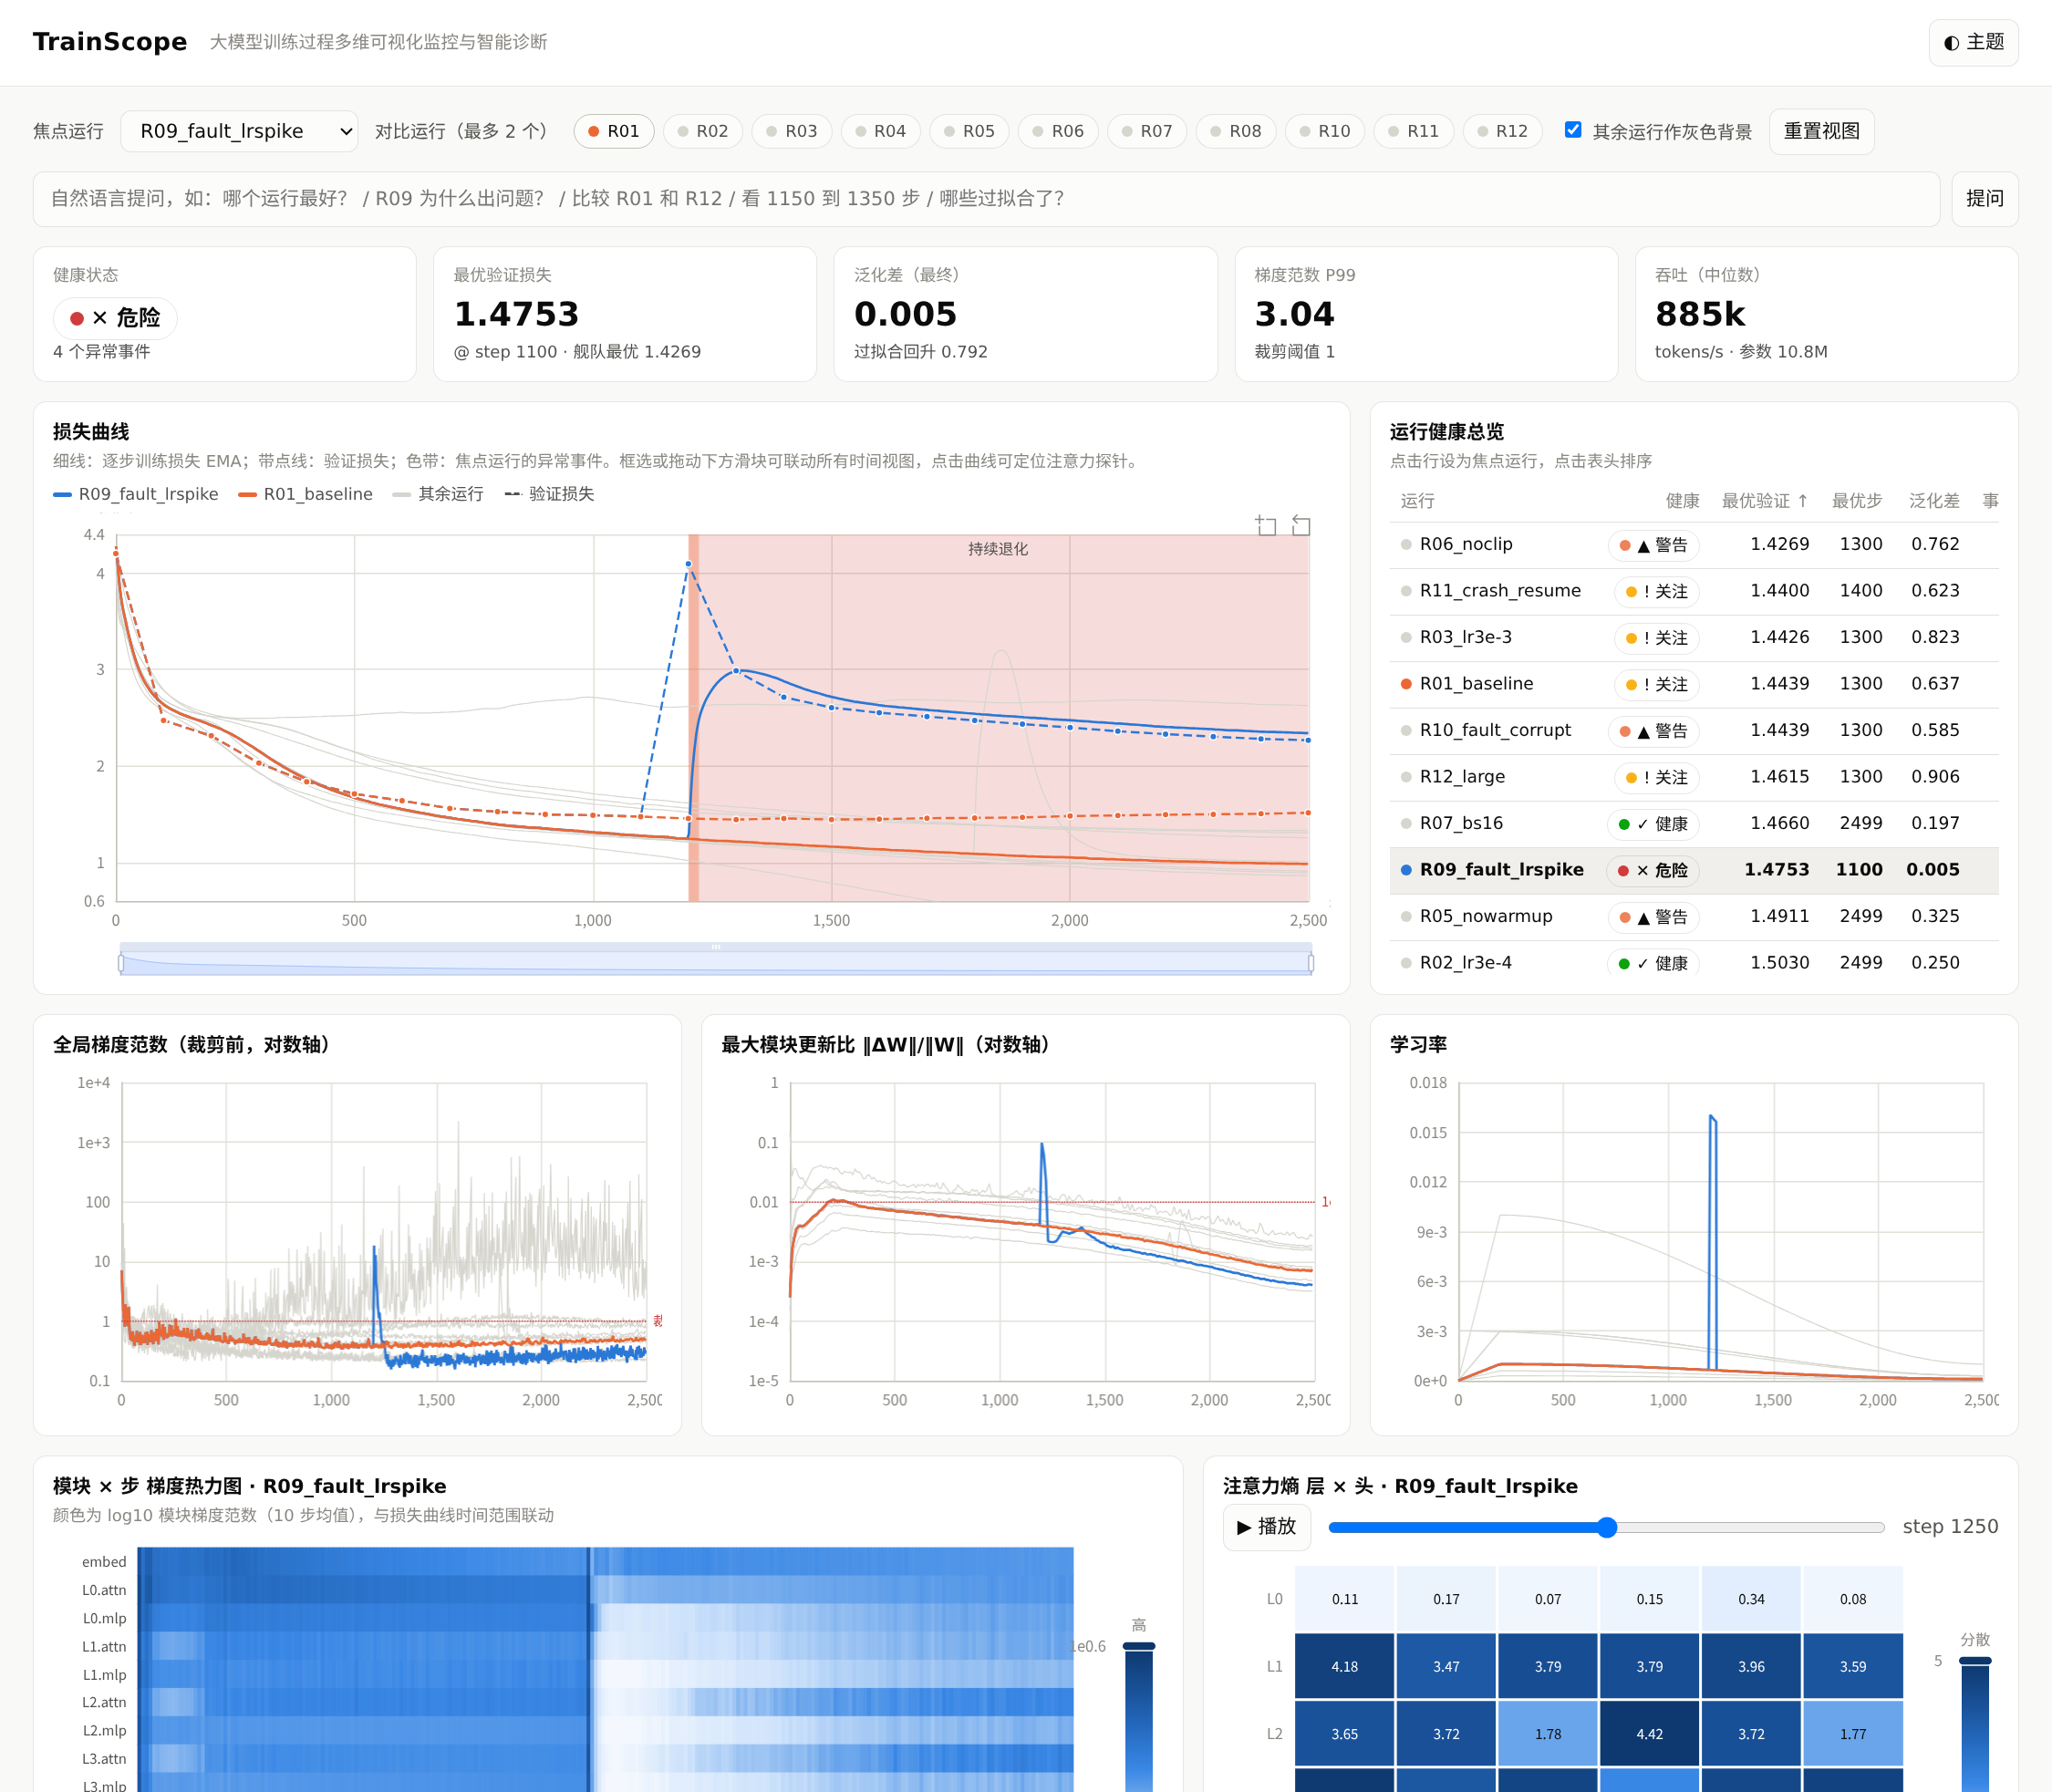
\includegraphics[width=\linewidth]{figures/dash_overview.png}
\caption{TrainScope 仪表盘首屏（焦点 R09，对比 R01）：控制栏、自然语言问答、KPI 磁贴、联动时间视图与运行健康总览}
\end{figure}

\begin{table}[htbp]
\centering
\caption{各运行结果与智能体诊断摘要}
\small
\begin{tabularx}{\linewidth}{XcccccX}
\toprule
\textbf{运行} & \textbf{最优验证} & \textbf{最优步} & \textbf{最终验证} & \textbf{泛化差} & \textbf{健康} & \textbf{主要事件 $\rightarrow$ 首要根因} \\
\midrule
R06\_noclip & 1.4269 & 1300 & 1.5544 & 0.762 & 警告 & 梯度爆炸@172 $\rightarrow$ 未启用裁剪；过拟合 \\
R11\_crash\_resume & 1.4400 & 1400 & 1.5016 & 0.623 & 关注 & 过拟合（续训本身无异常） \\
R03\_lr3e-3 & 1.4426 & 1300 & 1.5877 & 0.823 & 关注 & 过拟合 \\
R01\_baseline & 1.4439 & 1300 & 1.5146 & 0.637 & 关注 & 过拟合 \\
R10\_fault\_corrupt & 1.4439 & 1300 & 1.4954 & 0.585 & 警告 & 损失尖峰@1800 $\rightarrow$ 数据管道污染（98\%） \\
R12\_large & 1.4615 & 1300 & 1.6394 & 0.906 & 关注 & 过拟合 $\rightarrow$ 容量过剩（88\%） \\
R07\_bs16 & 1.4660 & 2499 & 1.4660 & 0.197 & 健康 & — \\
R09\_fault\_lrspike & 1.4753 & 1100 & 2.2669 & 0.005 & 危险 & 尖峰@1200 $\rightarrow$ 学习率异常（99\%）；持续退化 \\
R05\_nowarmup & 1.4911 & 2499 & 1.4911 & 0.325 & 警告 & 注意力塌缩@450–1400 $\rightarrow$ 缺少预热（79\%） \\
R02\_lr3e-4 & 1.5030 & 2499 & 1.5030 & 0.250 & 健康 & — \\
R08\_nodropout & 1.5179 & 900 & 3.1976 & 2.997 & 关注 & 过拟合@1100 $\rightarrow$ 容量过剩/无 dropout（92\%） \\
R04\_lr1e-2\_noclip & 2.4691 & 200 & 2.5191 & $-$0.003 & 警告 & 停滞、注意力塌缩 $\rightarrow$ 学习率过高；梯度爆炸 $\rightarrow$ 未裁剪 \\
\bottomrule
\end{tabularx}
\end{table}

图 5 用 3$\times$4 小多图同时展示 12 个运行的训练/验证损失和异常色带。小多图让每个运行拥有独立的坐标系，避免 12 条曲线叠在一起；所有子图共享 x、y 轴范围，因此可以直接比较。从图中可以一眼看出四种“曲线形态”：健康收敛（R02、R07）、收敛后过拟合（R01、R03、R06、R08、R12）、整体停滞（R04）和突发断裂（R09、R10）。

\begin{figure}[htbp]
\centering
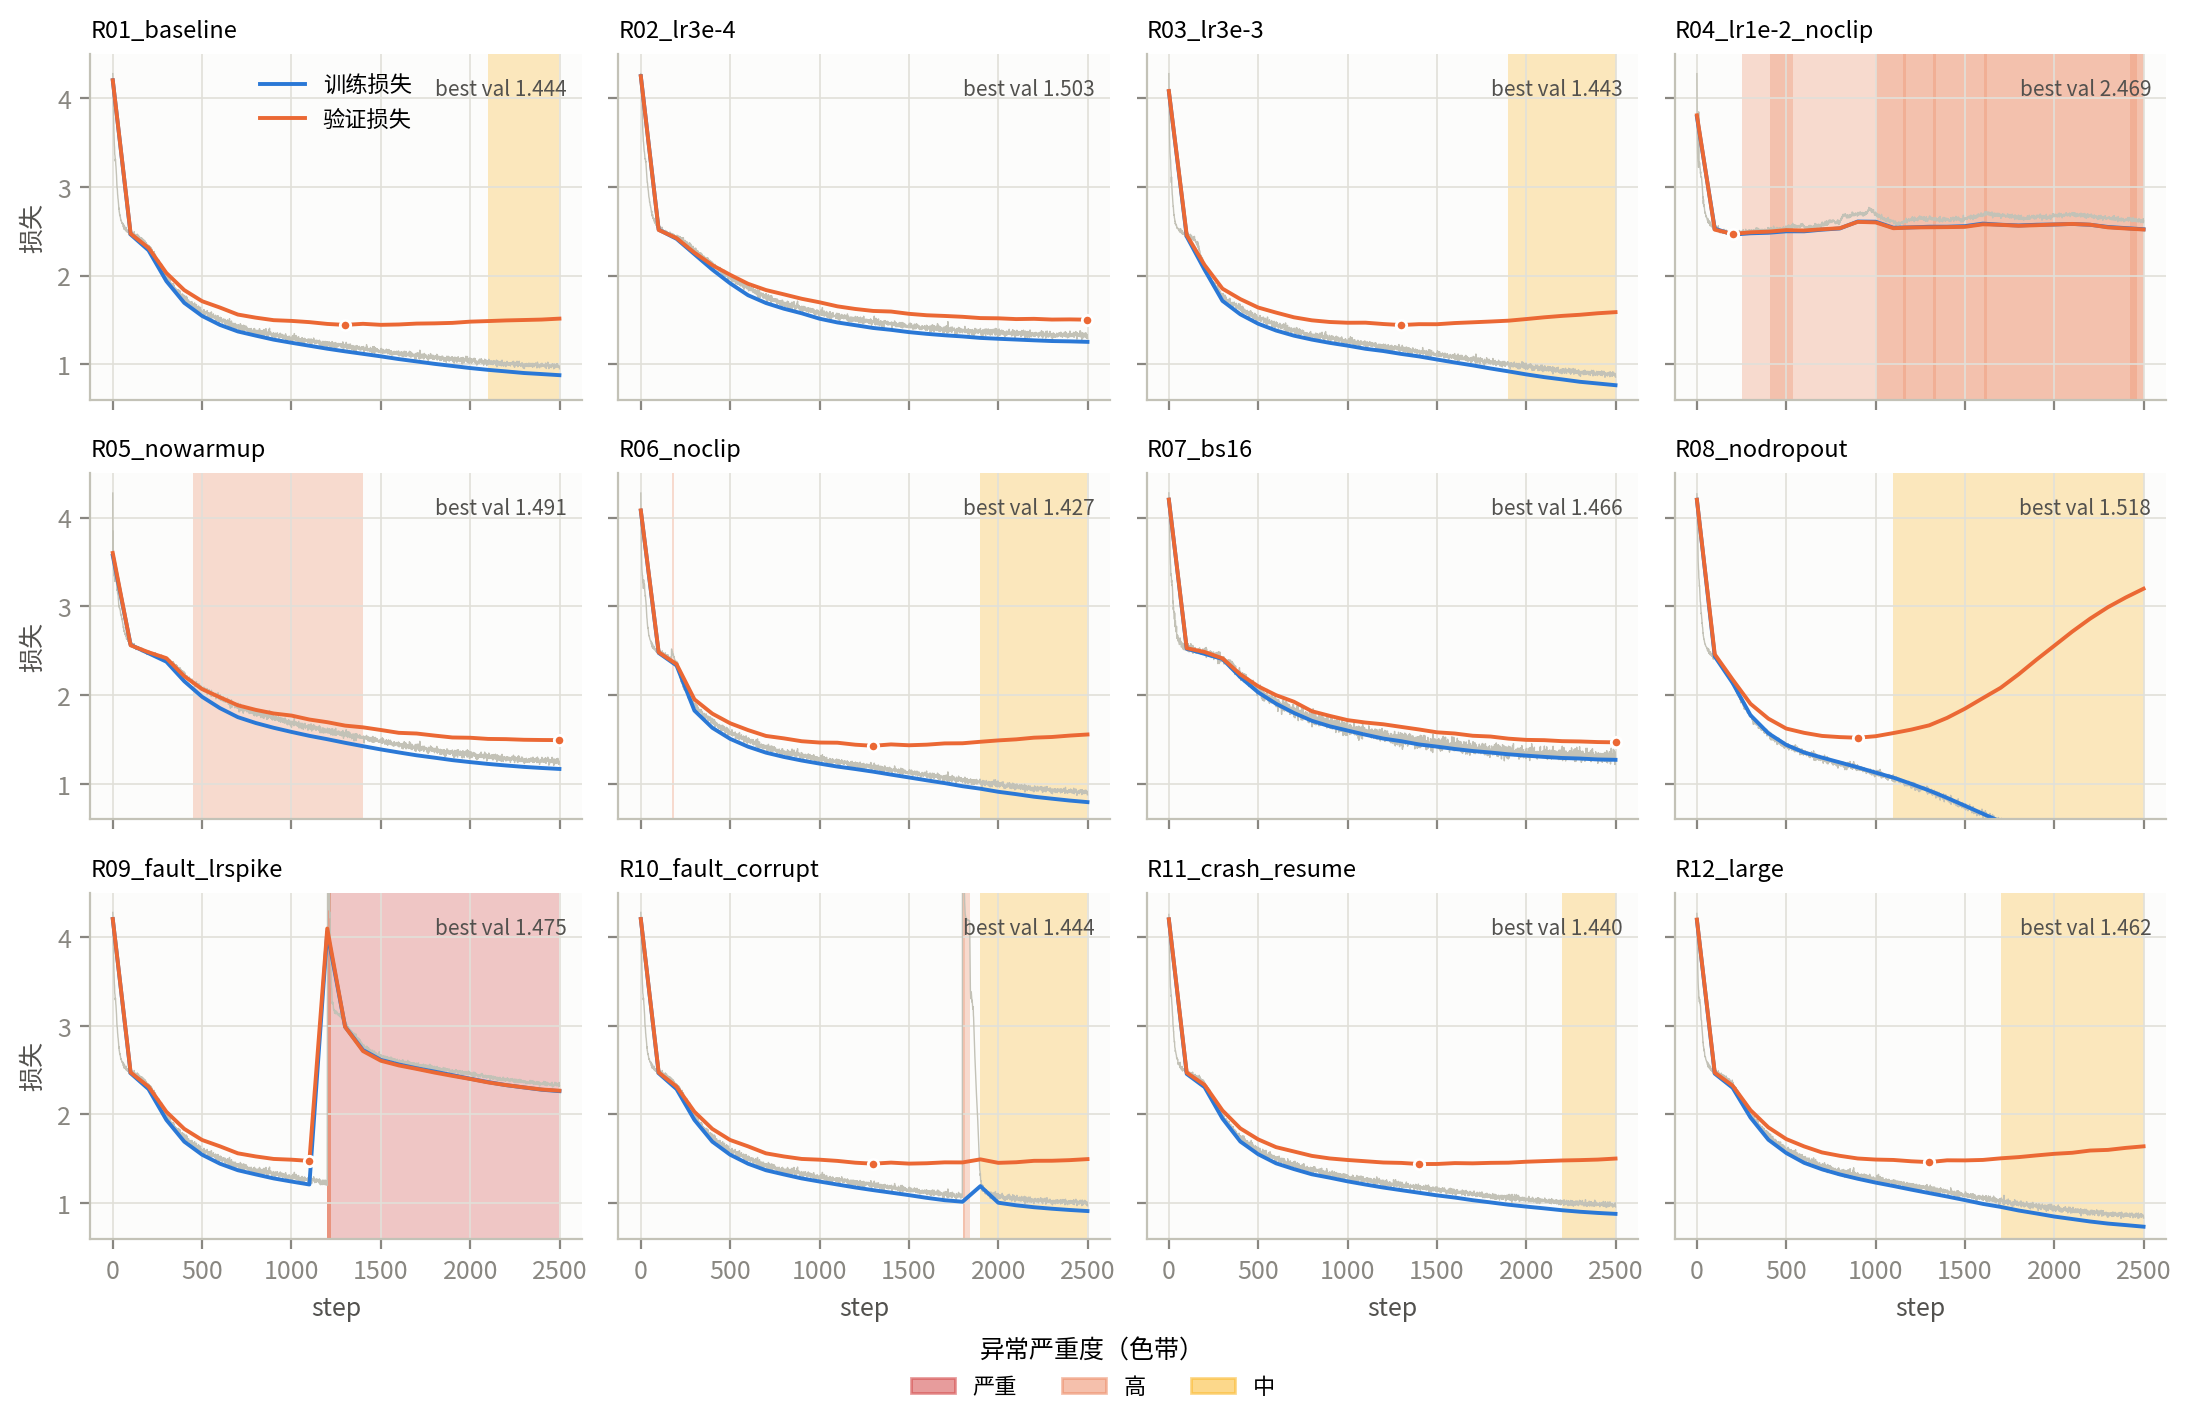
\includegraphics[width=\linewidth]{figures/fig_small_multiples.png}
\caption{12 个运行的损失小多图（蓝：训练，橙：验证，灰：逐步训练损失，圆点：最优验证点，色带：检测到的异常事件）}
\end{figure}

\subsection{故障案例一：学习率尖峰的“不可逆损伤”}

R09 在第 1200–1229 步把学习率放大了 25 倍（约 2.4e-2）。如图 7(a)，异常前训练损失约为 1.23，注入后逐步损失在 20 步内冲到 6.93，梯度范数从约 0.35 升到 18.5，最大模块更新比从 4.3e-3 跃升到 3.1e-2，超过了 1e-2 的经验上限。\textbf{关键发现是损伤不可逆}：学习率在第 1230 步恢复正常后，验证损失从 4.09（第 1200 步）只回落到 2.99（第 1300 步）、2.40（第 2000 步）和 2.27（第 2499 步），在剩下的 1270 步中都没有回到注入前的 1.48，相当于把模型打回了“二元语法”水平（约 2.5 nats）。

图 6(b) 的模块热力图解释了原因：注入之后，L0.mlp 到 L5.mlp 的中间层梯度下降了 1–2 个数量级（热力图中呈现近乎白色的条带），而 embed 和 head 两端的梯度仍保持原来的量级。这说明中间层已经进入饱和或“死亡”状态，模型基本上只靠嵌入层和输出层做浅层预测，所以损失停在 n-gram 统计的水平。PCA 轨迹视图（图 12(a)）也从另一个角度印证了这一点：R09 的轨迹在第 1200 步突然向 PC1 负方向跳跃了约 12 个单位，离开了健康运行所在的区域，之后再也没有回来。由于 PC1 的载荷在 12 个中间模块上几乎相等（约 0.3），它可以理解为“网络整体梯度强度”，这一跳跃正是中间层梯度坍缩的低维投影。

智能体的诊断如图 8 所示。Monitor 在第 1200 步（零延迟）同时报告了损失尖峰、梯度爆炸、更新比跃升和持续退化 4 个事件。Diagnostician 的取证工具测得事件窗口学习率是前序窗口的 12.9 倍、更新比升至 1.8e-2、验证损失同步上升 0.20，因此以 99\% 的置信度判定为“学习率过高/调度异常”。对于持续退化事件，它把时间上相关联的前序冲击纳入证据，判定为“前序冲击造成的不可逆损伤”（86\%）。Advisor 给出两条建议：检查调度器配置，以及终止当前运行、回滚到第 1100 步（验证最优）的检查点。按本实验的数据计算，如果在第 1230 步就采纳这条建议，可以节省剩余 51\% 的训练算力，并保住 1.4753 的验证损失，而不是最终的 2.2669。

\begin{figure}[htbp]
\centering
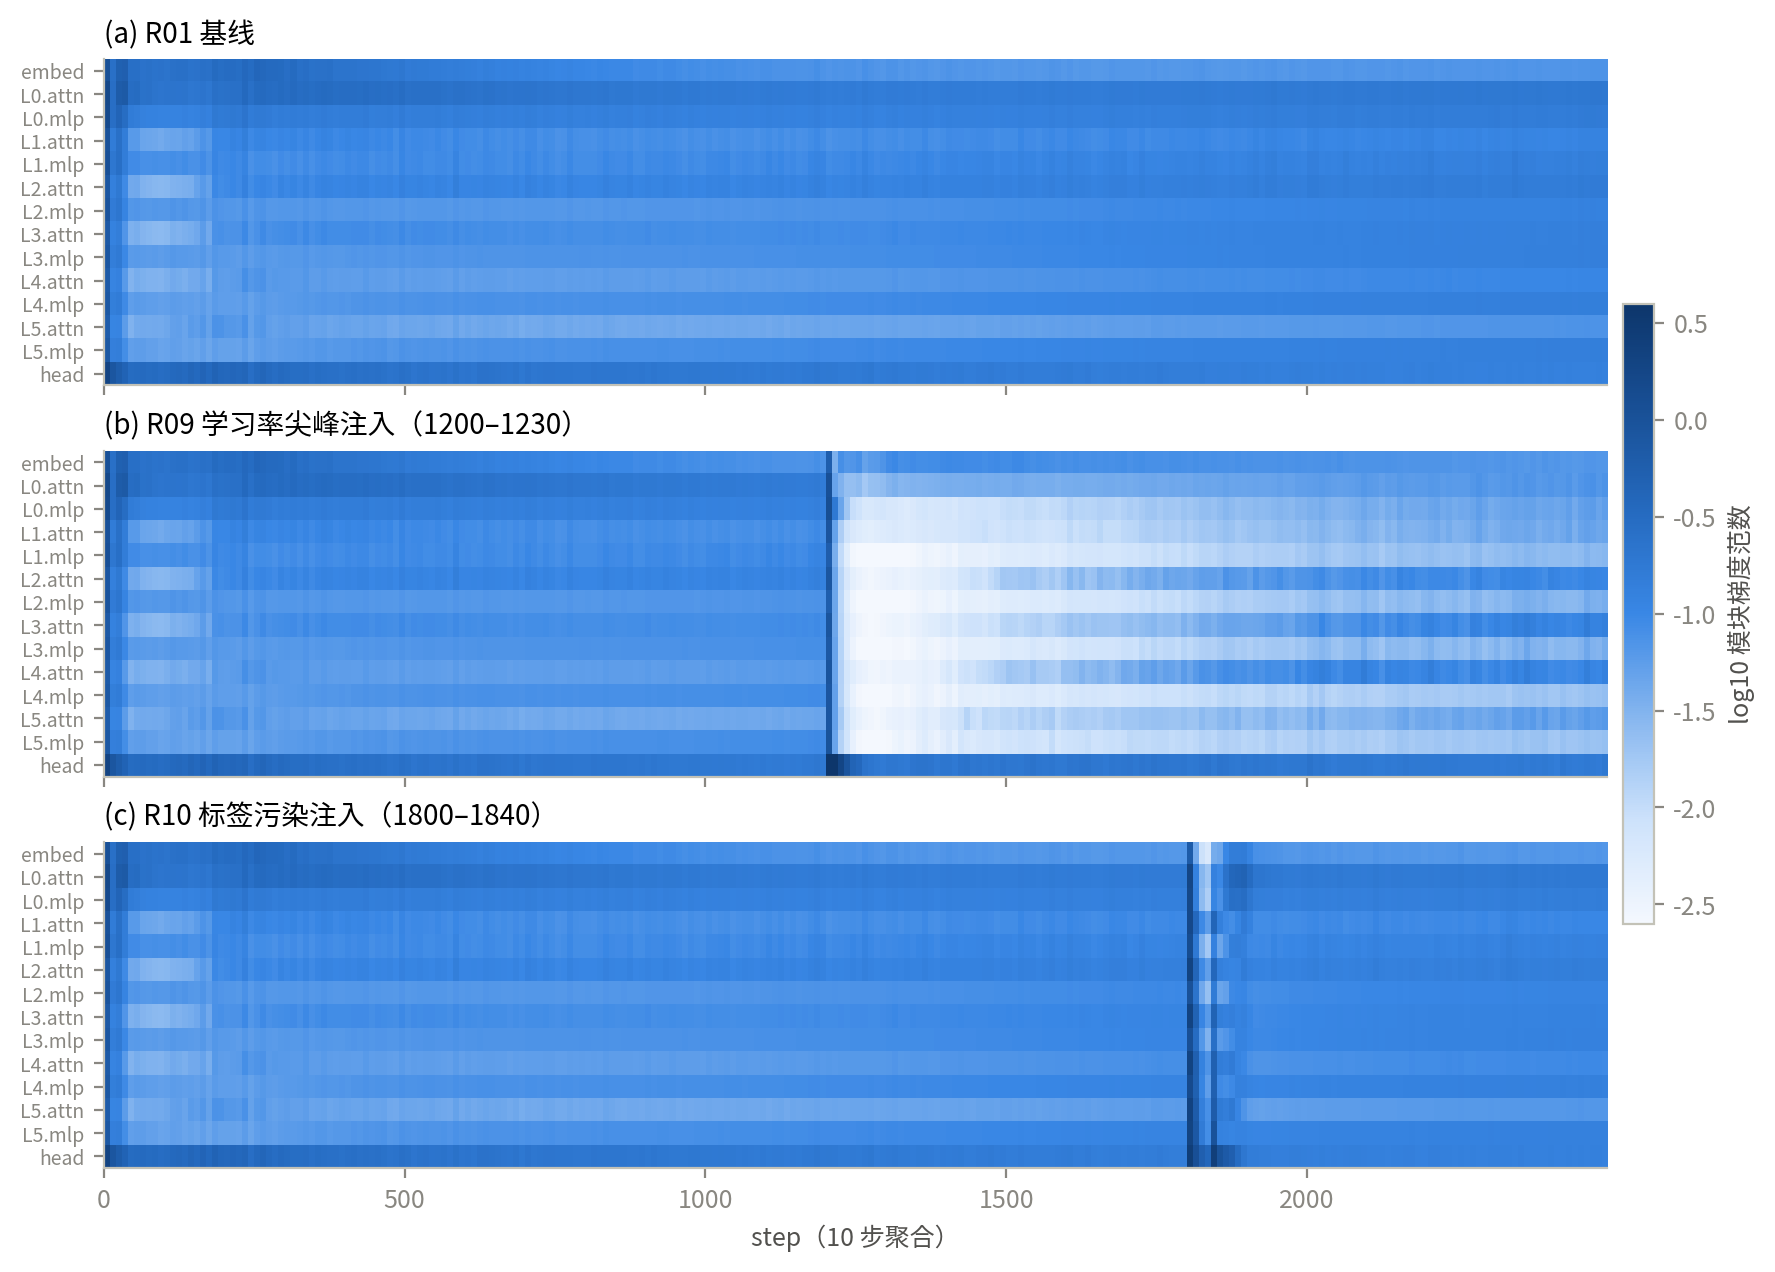
\includegraphics[width=\linewidth]{figures/fig_module_heatmap.png}
\caption{模块$\times$步梯度热力图（log10，10 步聚合）：(a) 基线；(b) 学习率尖峰后中间层梯度坍缩；(c) 标签污染期间全模块梯度短暂增强后完全恢复}
\end{figure}

\subsection{故障案例二：数据污染与学习率问题的区分}

R10 在第 1800–1839 步把标签替换为随机字符。从损失曲线看，它和 R09 一样是一个巨大的尖峰（峰值 11.50，甚至比 R09 更高），只看曲线很容易误判为学习率问题。但多视图联动给出了完全不同的证据（图 7(b)）：

\begin{itemize}
\item \textbf{学习率与更新比没有变化}：学习率比值为 0.81（余弦衰减造成的自然下降），开启了裁剪的更新比只从 2.2e-3 小幅波动到 2.6e-3，远低于 R09 的 3.1e-2；
\item \textbf{损失高于随机猜测}：峰值 11.50 远大于 ln65=4.17，而污染期间的平均损失 4.19 恰好接近 ln65，说明模型在几十步内就“学会”了对随机标签输出接近均匀的分布；
\item \textbf{验证损失几乎不动}：验证损失从 1.458（第 1800 步）只变化到 1.493（第 1900 步），随后在第 2000 步回到 1.453。验证集作为“未受污染的对照组”表明权重没有受到实质性损伤；
\item \textbf{模块热力图显示“全面、短暂、可恢复”}：图 6(c) 中所有模块在第 1800 步同时变深（梯度增强），在第 1840 步后迅速恢复为与基线一致的条纹模式。这与 R09 的“中间层永久坍缩”形成鲜明对比。
\end{itemize}

知识库据此以 98\% 的置信度判定为“数据管道污染”，建议“隔离第 1800–1841 步对应的数据分片，校验 tokenizer/标签对齐与样本哈希；该段损失无需回滚”。这条建议与 R09 的“回滚”建议完全不同，体现了根因区分对实际决策的价值：对 R10 而言回滚是不必要的，平滑训练损失在第 2052 步就回到了污染前的水平，最终验证损失（1.4954）与基线（1.5146）相当，甚至略好。图 9 展示了用户在问答框中输入“R10 为什么出问题？”之后的界面：系统自动把焦点切换到 R10，把四个时间视图缩放到 1600–2091 步，并把注意力探针定位到第 1800 步，同时在回答框中列出事件、根因、置信度和建议。

\begin{figure}[htbp]
\centering
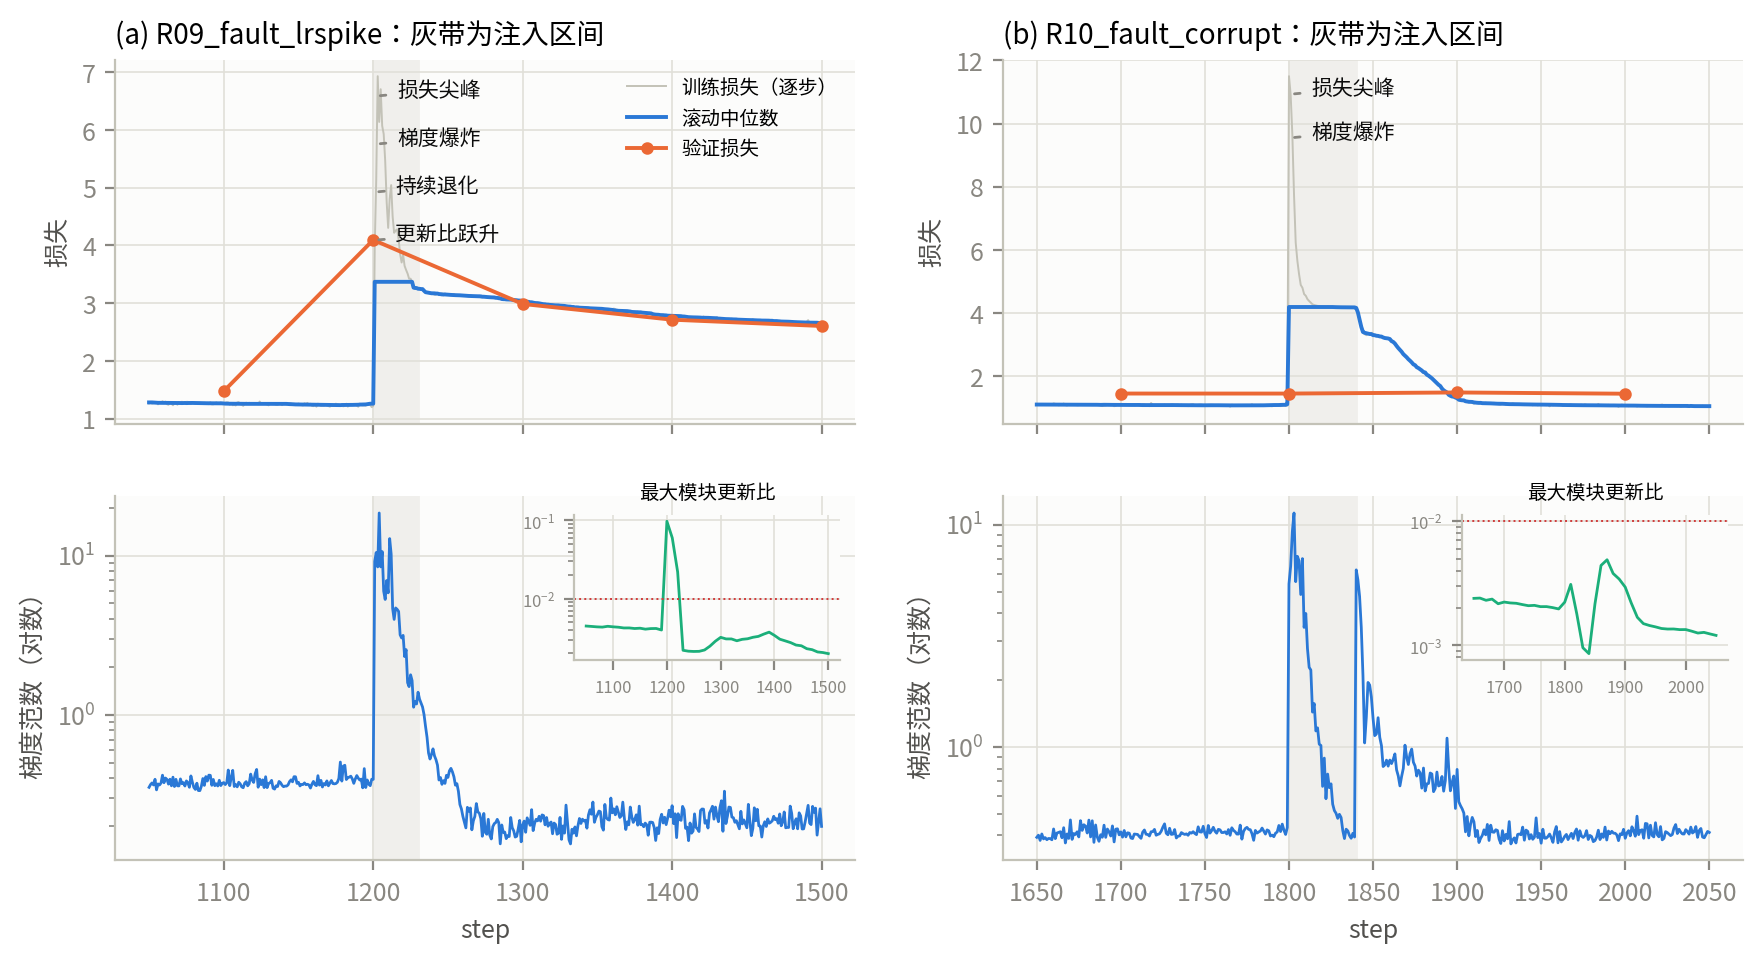
\includegraphics[width=\linewidth]{figures/fig_detection.png}
\caption{注入故障的放大视图（灰带为真实注入区间）：(a) R09 学习率尖峰；(b) R10 标签污染。下排为梯度范数，嵌入小图为最大模块更新比（红色虚线为 1e-2）}
\end{figure}

\begin{figure}[htbp]
\centering
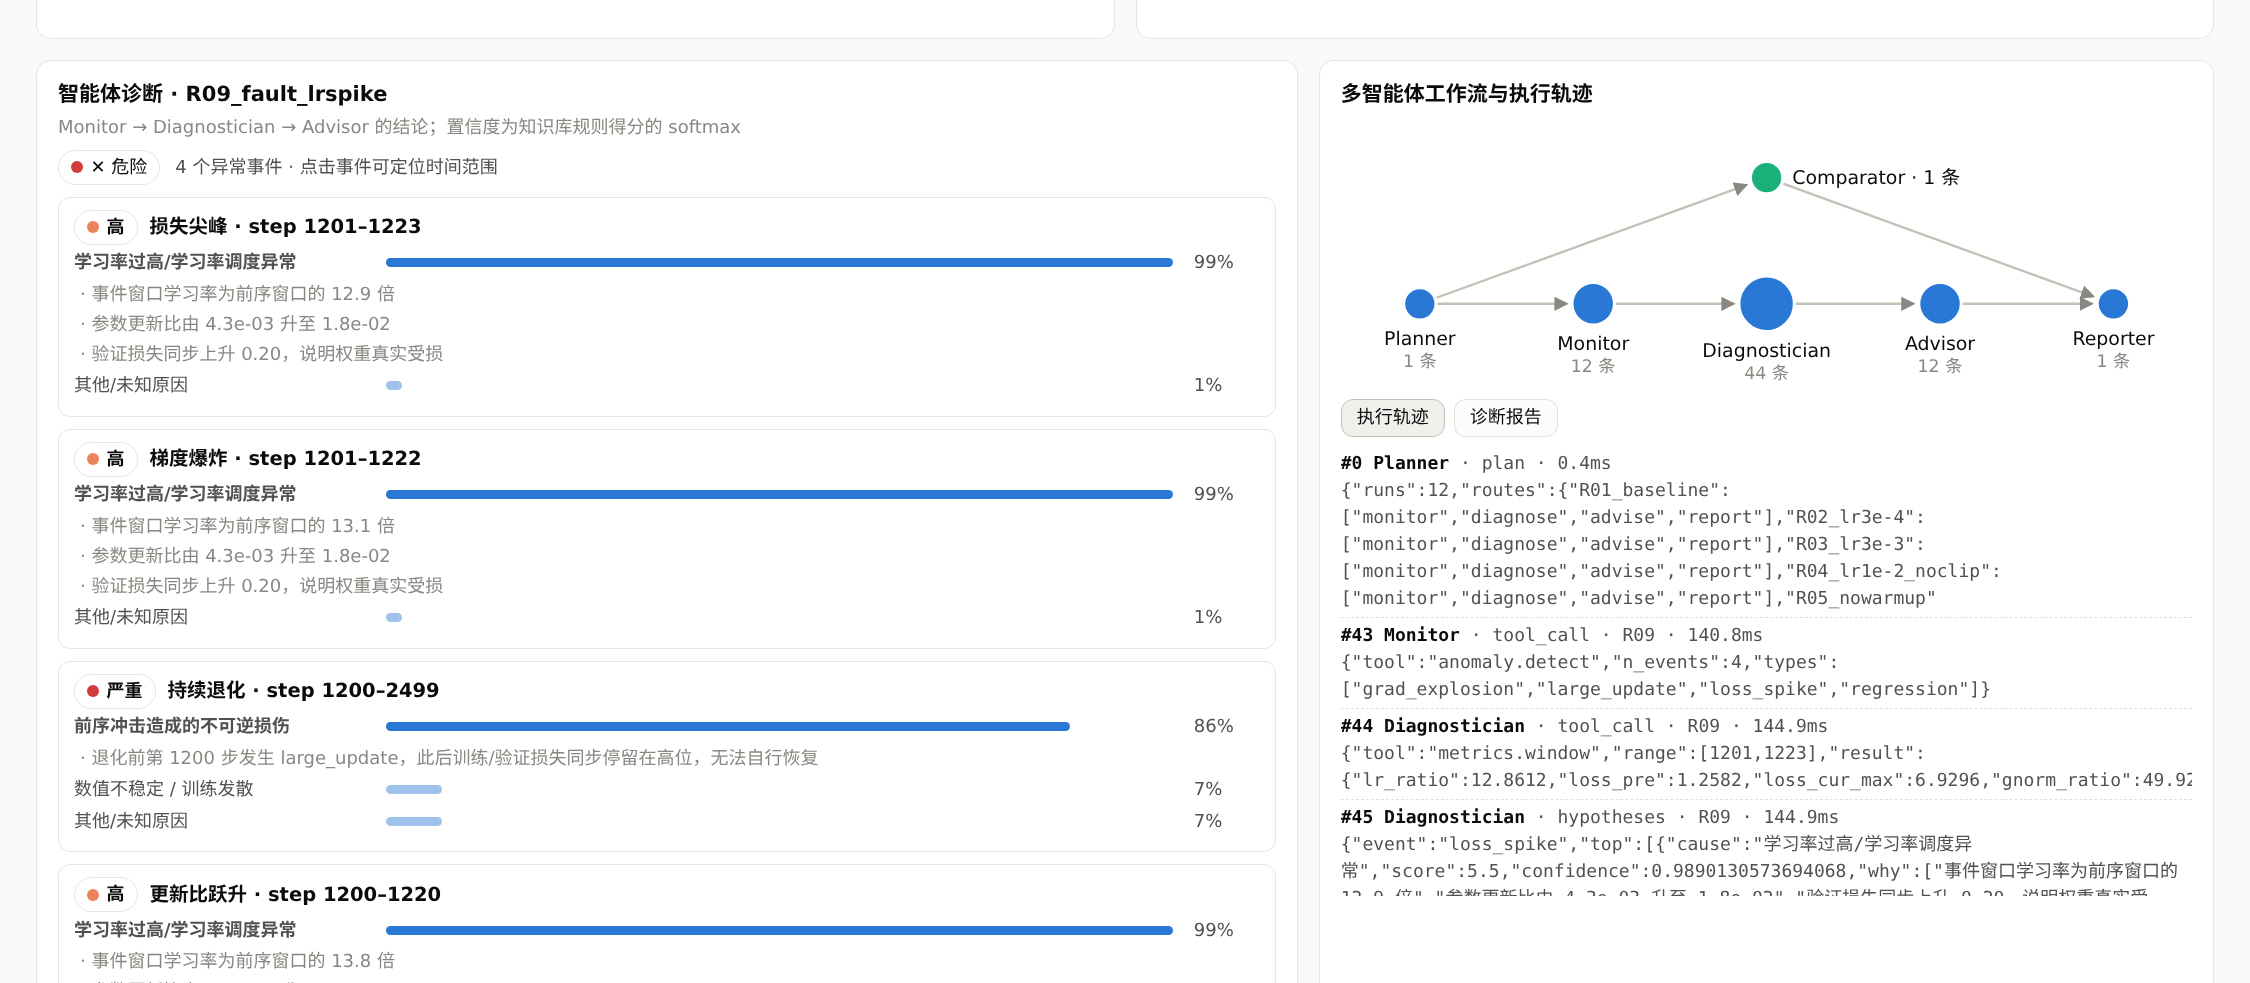
\includegraphics[width=\linewidth]{figures/dash_agent.png}
\caption{智能体诊断面板（R09）：事件卡片、根因置信度条与依据、处置建议，以及多智能体工作流节点图（节点大小表示消息数）和可回放的执行轨迹}
\end{figure}

\begin{figure}[htbp]
\centering
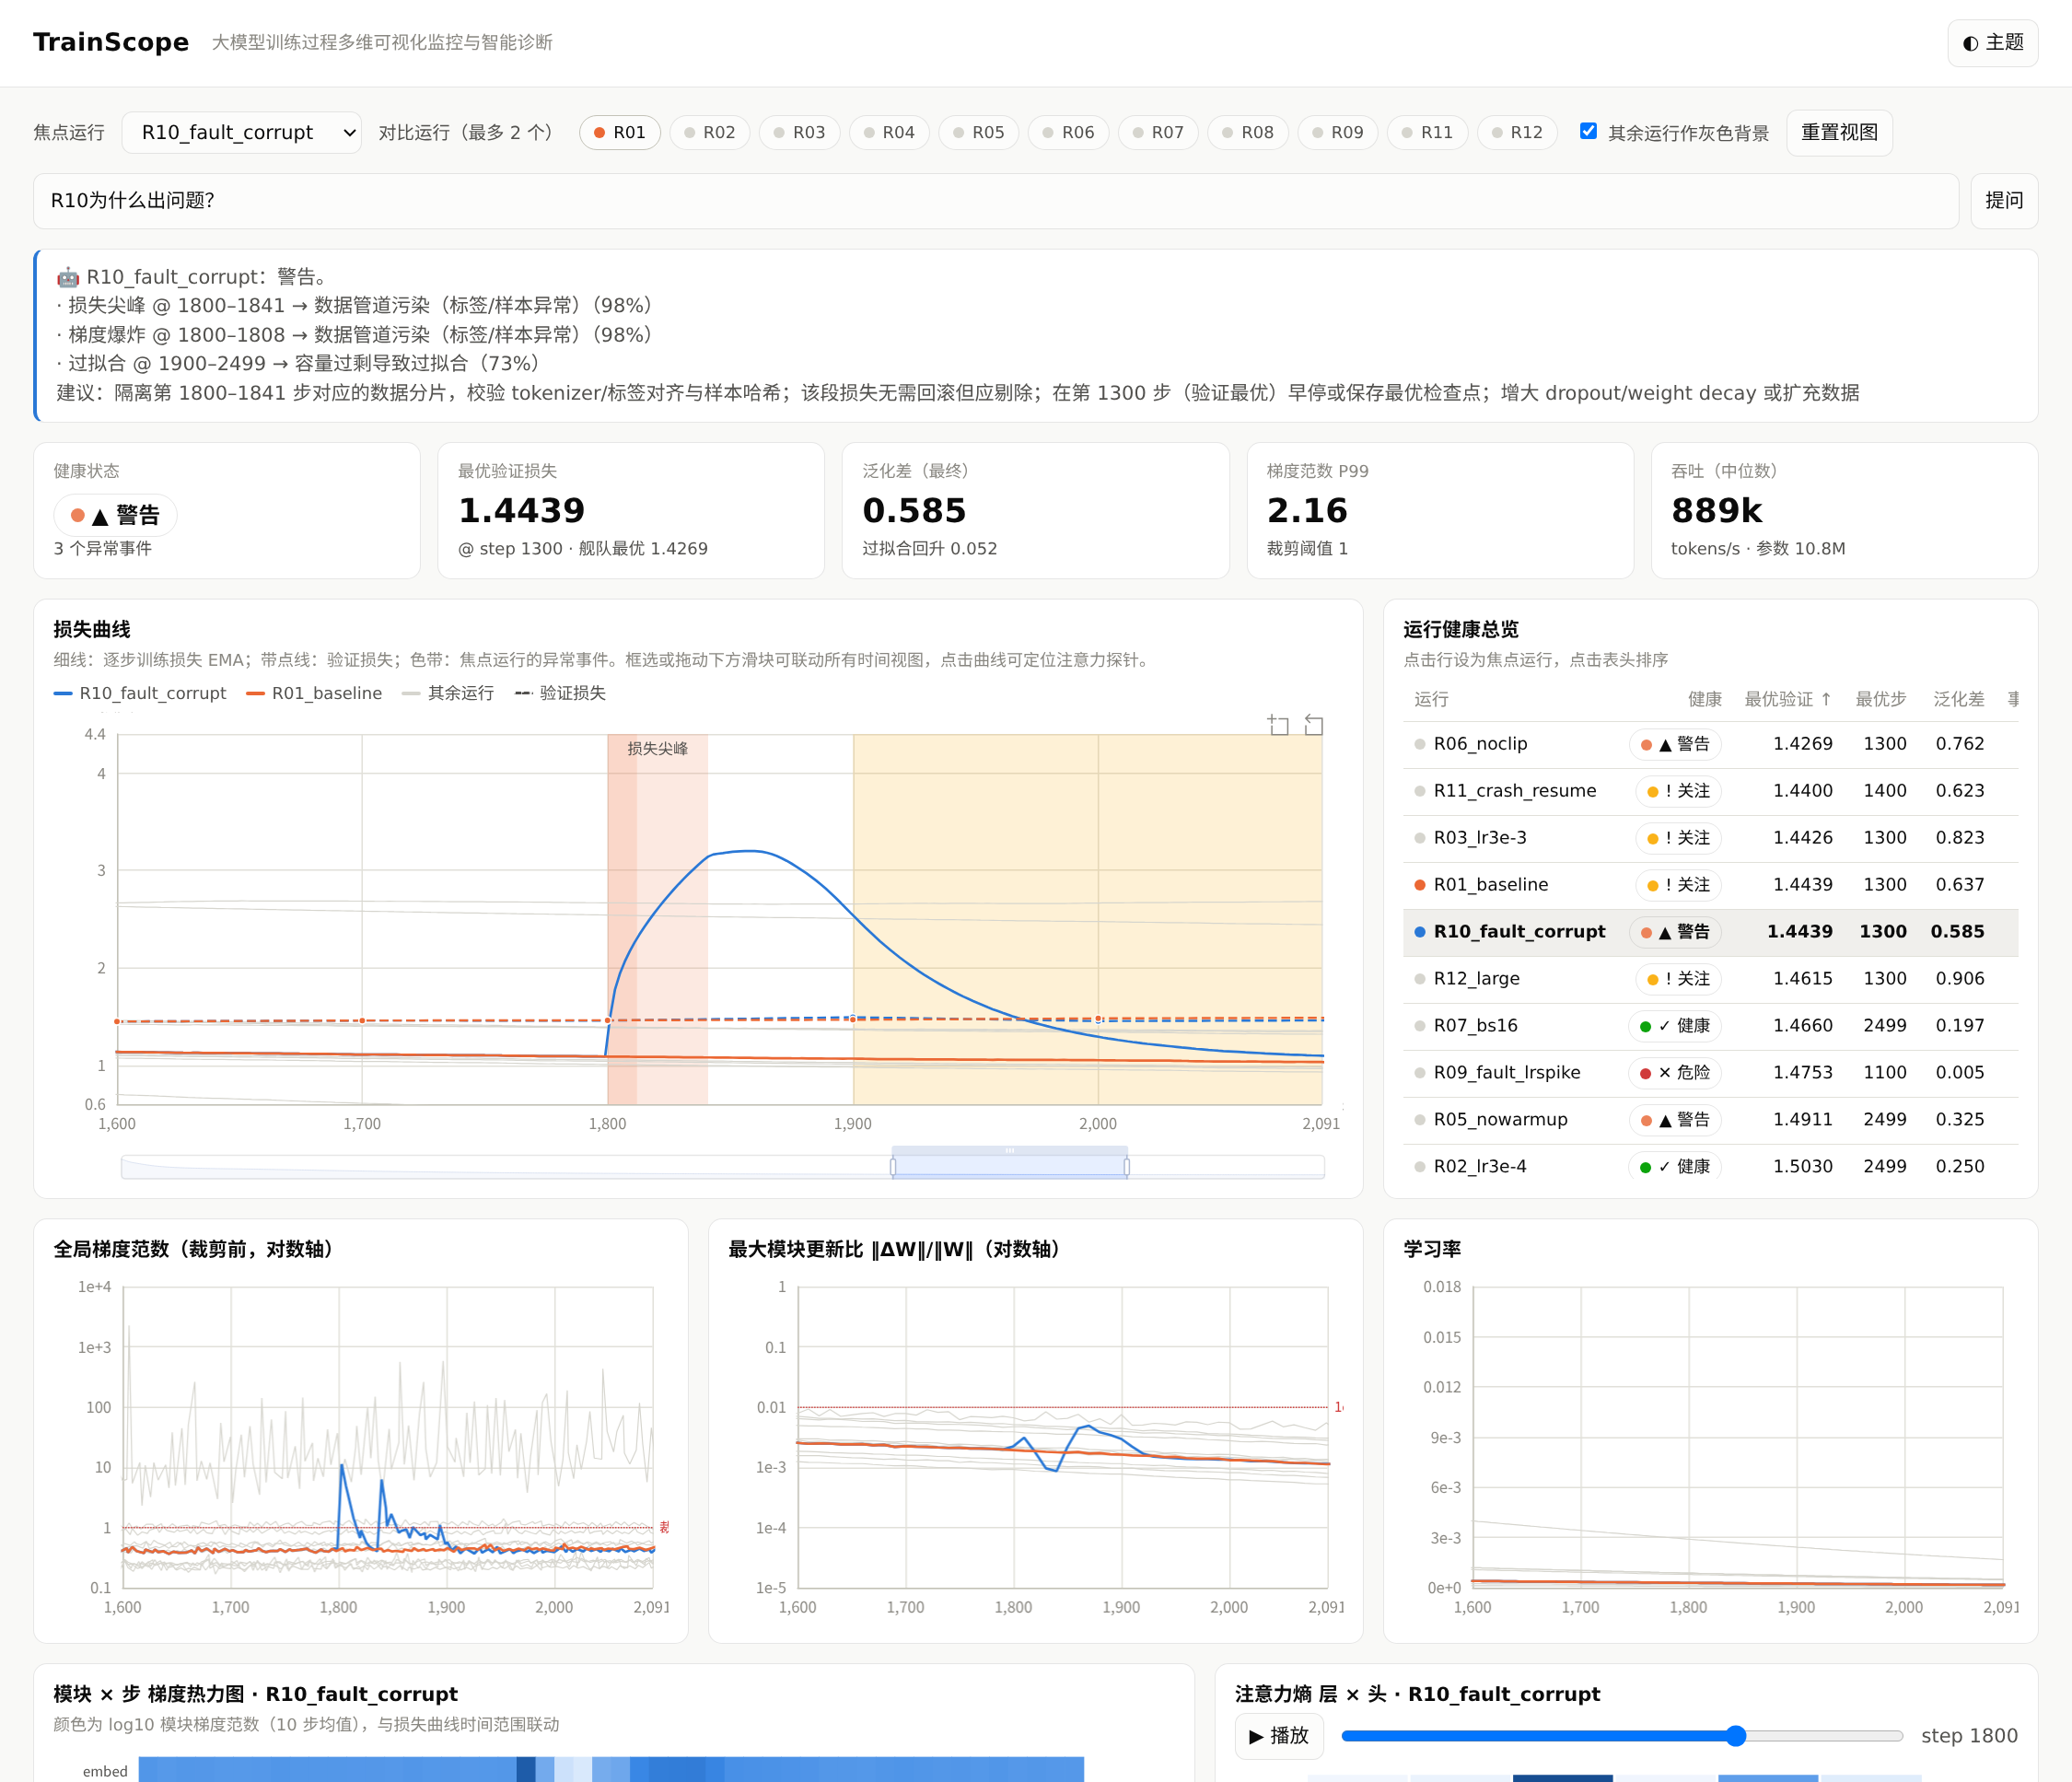
\includegraphics[width=\linewidth]{figures/dash_q_r10.png}
\caption{自然语言交互：提问“R10 为什么出问题？”后，系统自动聚焦、联动缩放到事件区间并给出带依据的回答}
\end{figure}

\subsection{异常检测的定量评估}

以注入故障的真实区间为真值，本文对 Monitor 做了事件级评估（表 8）。两个注入故障都在注入的第一步被检出（延迟 0 步），并且分别被 3 个和 2 个独立检测器同时命中，形成相互印证。在 6 个健康或仅有过拟合的运行（R01、R02、R07、R08、R11、R12）上，“突发类”检测器（尖峰、爆炸、跃升、发散、停滞、塌缩）的误报数为 0。全部 12 个运行共产生 22 个事件，其中 8 个梯度爆炸事件有 6 个来自不裁剪的 R04 与 R06，另外 2 个对应两次注入故障。合并间隔的设计也很重要：在 R04 中，第 411–540 步内相隔数十步的多次超阈值尖峰被归并为一个事件簇，否则同一个慢性问题会反复告警，造成告警疲劳。

\begin{table}[htbp]
\centering
\caption{注入故障的事件级检测结果}
\small
\begin{tabularx}{\linewidth}{XcccXX}
\toprule
\textbf{故障} & \textbf{真实区间} & \textbf{检出} & \textbf{延迟} & \textbf{命中检测器} & \textbf{首要根因（置信度）} \\
\midrule
学习率尖峰（R09） & 1200–1229 & \checkmark{} & 0 步 & loss\_spike, grad\_explosion, large\_update & 学习率异常（99\%） \\
标签污染（R10） & 1800–1839 & \checkmark{} & 0 步 & loss\_spike, grad\_explosion & 数据管道污染（98\%） \\
健康运行误报 & — & \multicolumn{2}{c}{0 次} & \multicolumn{2}{c}{6 个运行共 15,000 步} \\
\bottomrule
\end{tabularx}
\end{table}

需要客观说明的是，这一评估的规模很小（2 个注入故障），检测器阈值也是在同一数据上通过 EDA 调整的，存在过拟合于本数据集的风险。开发过程中本文也记录到了知识库的真实失败案例：早期版本把 R04 中孤立的梯度尖峰误判为“数据污染”（置信度 37\%），原因是“验证损失不变”这条规则在没有训练损失飙升的情况下也会触发；加上“峰值比前序高 1.0”的前置条件后才得到纠正。这说明规则知识库需要用更多故障样本做系统的回归测试。

\subsection{表征层洞察：注意力熵与预热}

注意力熵视图揭示了损失曲线上看不到的内部动态（图 10）。初始化时所有头的熵都约为 4.55 nats（接近均匀分布），在基线 R01 中，平均熵在前 300 步迅速下降到 2.92，之后缓慢稳定在 2.3 左右。到训练结束，L0 层出现了熵仅为 0.04–0.10 的 3 个“尖锐头”，它们几乎只关注单个位置，类似于文献中描述的“前一字符头”（previous-token head）\cite{r20}；而 L1 层的各个头保持了 3.5 以上的高熵，负责聚合较长的上下文。这种按层分工的“头特化”是健康训练的标志，因此本文的检测器只对“全局平均熵 < 0.5”的塌缩报警，而不会对单个低熵头报警。早期版本的检测器曾因单头低熵对几乎所有运行误报，这是 EDA 修正的又一个例子。

\begin{figure}[htbp]
\centering
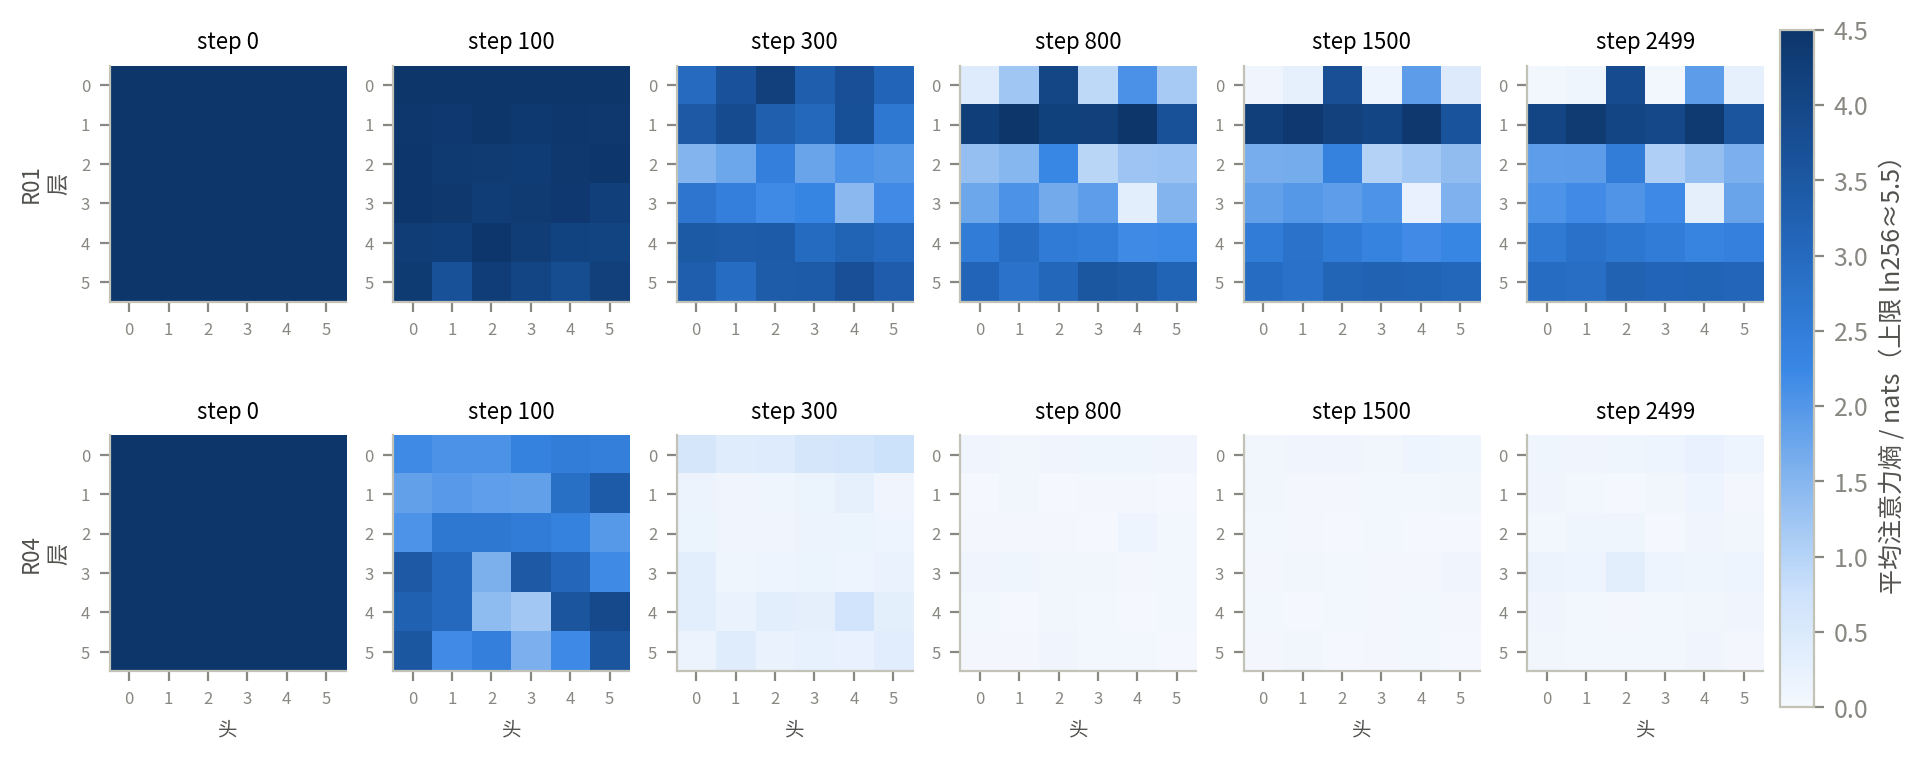
\includegraphics[width=\linewidth]{figures/fig_attention.png}
\caption{层$\times$头平均注意力熵的演化：上排为基线 R01（逐步特化），下排为 R04（学习率 1e-2，全局塌缩）}
\end{figure}

与基线相比，R04 的平均熵在 300 步内就塌缩到 0.27，此后一直低于 0.1，所有头都只关注单个位置，模型因此无法利用上下文，损失停在 2.5 附近（停滞）。更有启发的是 R05（去掉预热，其余与 R03 相同）：平均熵在第 100 步降到 1.33，第 800 步降到 0.36，触发了“注意力塌缩”告警（第 450–1400 步）；但它没有像 R04 那样一直停滞，在学习率按余弦衰减的过程中，熵逐渐恢复到第 2499 步的 1.26，最终验证损失达到 1.491，代价是收敛明显变慢（R03 在第 1300 步就达到 1.443）。图 11 是暗色主题下仪表盘对 R05 的分析画面：通过“看 300 到 1600 步”的问句完成缩放，注意力视图显示第 300 步时 L1–L5 层大部分头的熵已低于 1。这一现象与 Zhai 等人提出的“注意力熵塌缩”\cite{r17}以及 Wortsman 等人在小模型上复现的“注意力 logit 增长”不稳定性\cite{r19}相吻合：没有预热时，训练初期以峰值学习率更新 Q/K 投影，注意力 logits 迅速增大，softmax 进入饱和区。预热的作用正是在 logits 尺度稳定之前限制更新幅度\cite{r18}。智能体以 79\% 的置信度把这一事件归因为“缺少学习率预热”，与文献结论一致。

\begin{figure}[htbp]
\centering
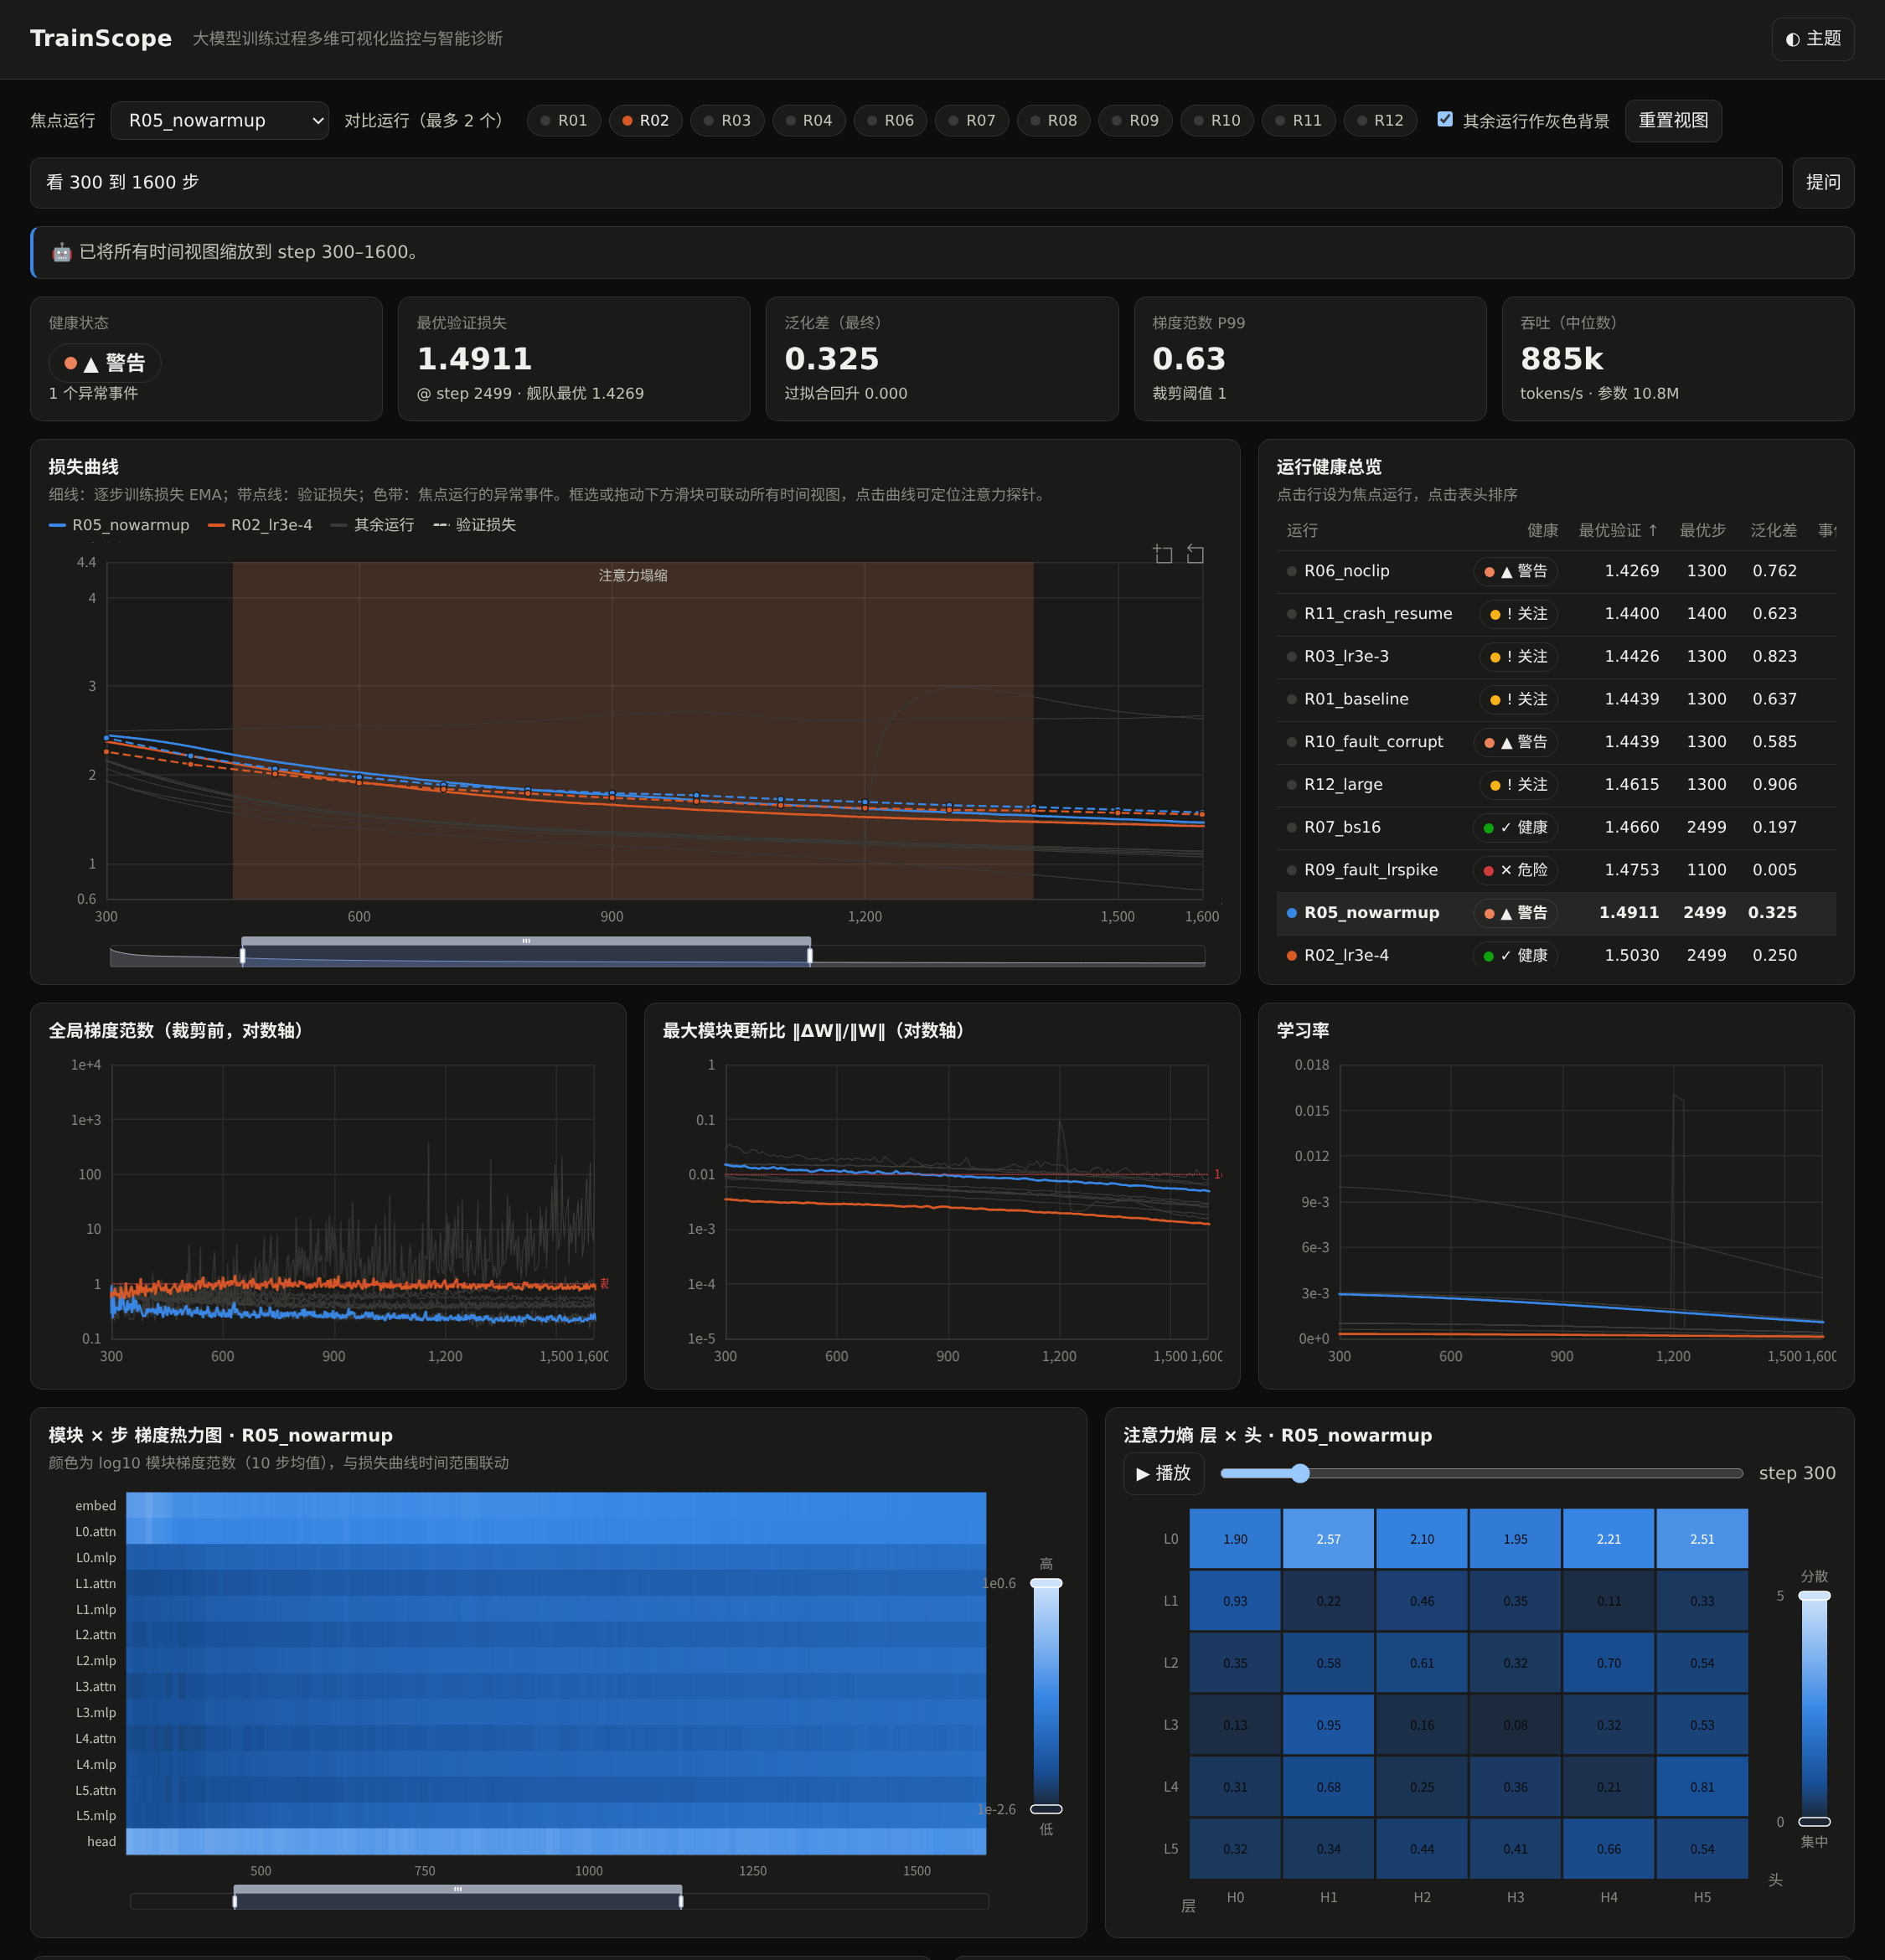
\includegraphics[width=\linewidth]{figures/dash_dark.png}
\caption{暗色主题下的 R05（无预热）分析：自然语言缩放到 300–1600 步，注意力塌缩色带与层$\times$头熵热力图}
\end{figure}

\subsection{降维视图的洞察}

\textbf{训练状态轨迹}。图 12(a) 中，PC1 与 PC2 共解释了 14 维模块梯度空间 89.0\% 的方差（69.4\% 与 19.6\%）。由图 12(b) 的载荷可知，PC1 在 12 个中间模块上的载荷近乎相等，代表“整体梯度强度”；PC2 的载荷由 embed/L0.attn（+0.55 以上）与深层/head（$-$0.1 至 $-$0.25）构成对比，代表“梯度在浅层与深层之间的分配”。健康运行的轨迹都从右侧起点出发，沿着一条狭窄的“走廊”向左下方缓慢移动，最终汇聚到相近的终点。R04 的轨迹先沿 PC2 正方向大幅上升到 +7，说明梯度高度集中在嵌入层和第一层注意力（与图 10 中 L0 的塌缩相互印证），然后在高位来回振荡，完全偏离了走廊。R09 的轨迹在注入点向 PC1 负方向剧烈跳跃。由此可见，一个 2D 轨迹视图就能把“健康/慢性异常/急性异常”三类训练形态区分开，非常适合作为大规模超参搜索时的概览视图。

\begin{figure}[htbp]
\centering
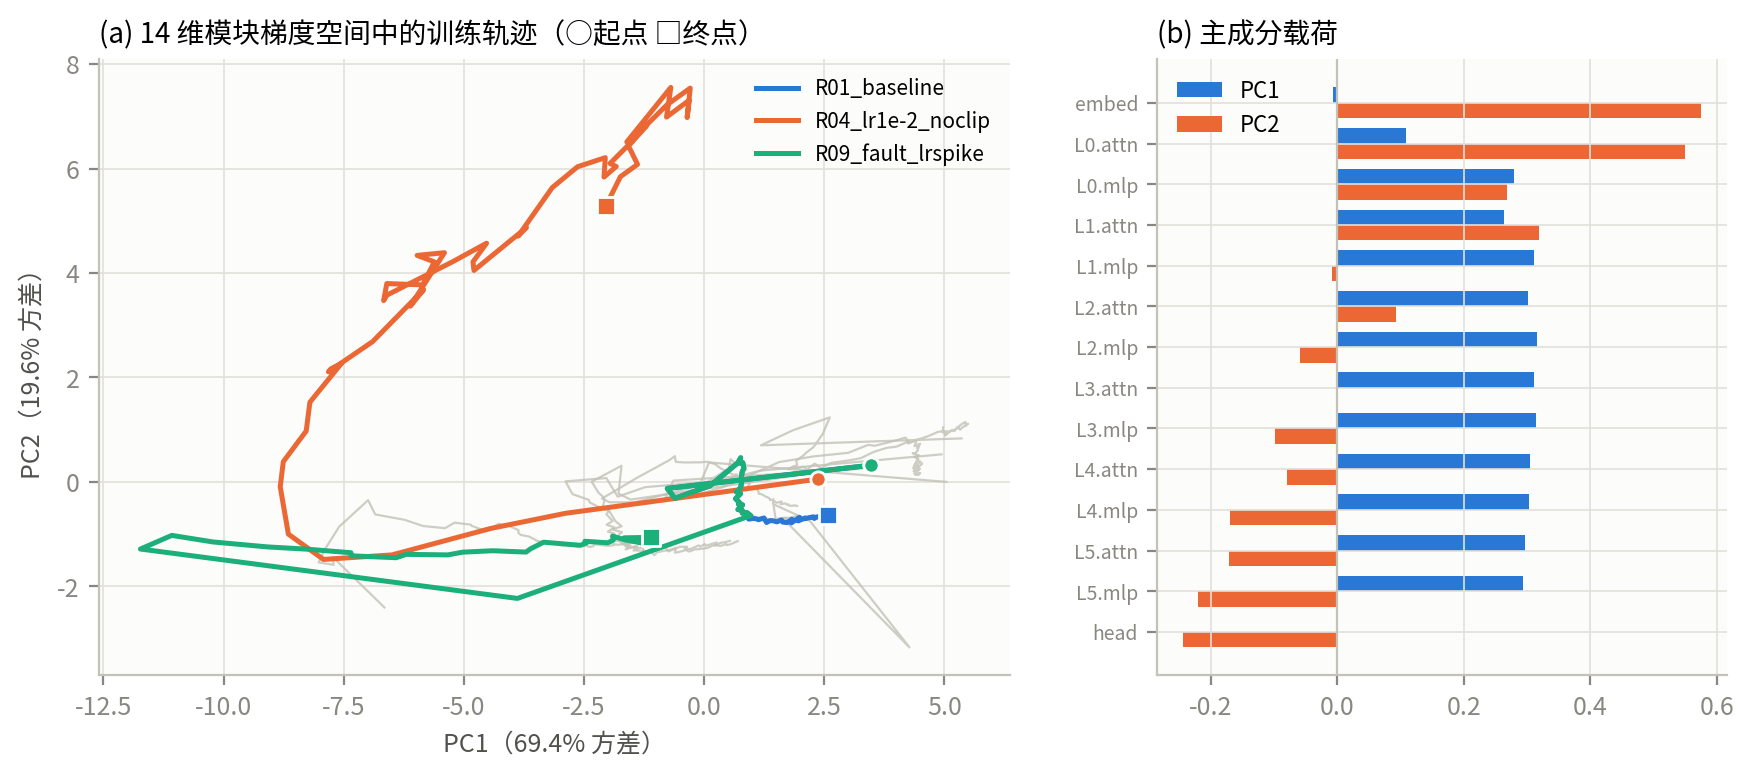
\includegraphics[width=\linewidth]{figures/fig_pca.png}
\caption{训练状态轨迹 PCA：(a) 11 个 6 层运行在模块梯度空间中的轨迹（灰色为其余运行）；(b) 前两个主成分的载荷}
\end{figure}

\textbf{字符嵌入空间}。对基线模型 65$\times$384 的字符嵌入做 t-SNE（图 13(b)），呈现出非常清晰的语义结构：标点符号（, ; : ? ! . -）聚在左上角；元音（a e i o u 及其大写）聚在中心；更有意思的是，\textbf{大小写字母成对出现}，如 b/B、d/D、s/S、m/M、h/H、k/K、j/J、q/Q 等在图中紧挨在一起。为了确认这不是 t-SNE 的投影假象，本文在原始 384 维空间中做了定量验证：26 对大小写字母的平均余弦相似度为 0.451，而全部字符对的平均值只有 0.017；在 26 个小写字母中，有 25 个（96.2\%）的最近邻正是自己的大写形式。也就是说，模型仅仅通过预测下一个字符，就自发学到了“大小写是同一个字母”这一抽象概念。相比之下，PCA 投影（图 13(a)）主要把大写字母与小写字母、标点分开，反映的是全局方差最大的方向：在剧本语料中，大写字母大多出现在行首和角色名中，上下文分布与小写字母差别最大。两种投影互为补充，也说明在需要揭示局部邻域结构时，t-SNE 比 PCA 更合适。

\begin{figure}[htbp]
\centering
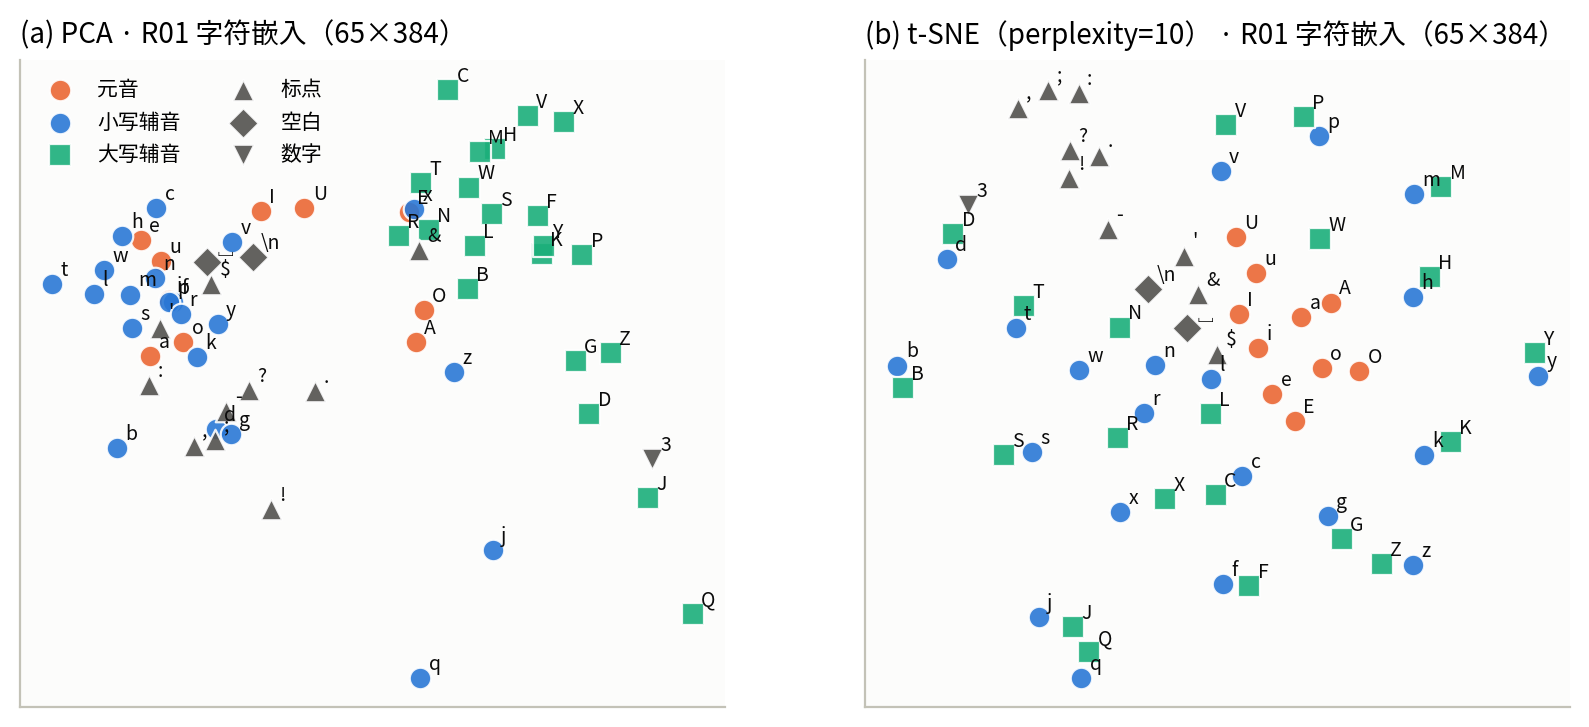
\includegraphics[width=\linewidth]{figures/fig_embed.png}
\caption{基线模型字符嵌入的二维投影：(a) PCA；(b) t-SNE。颜色与形状双重编码字符类别，每个点直接标注字符}
\end{figure}

\subsection{超参数规律与决策建议}

\begin{figure}[htbp]
\centering
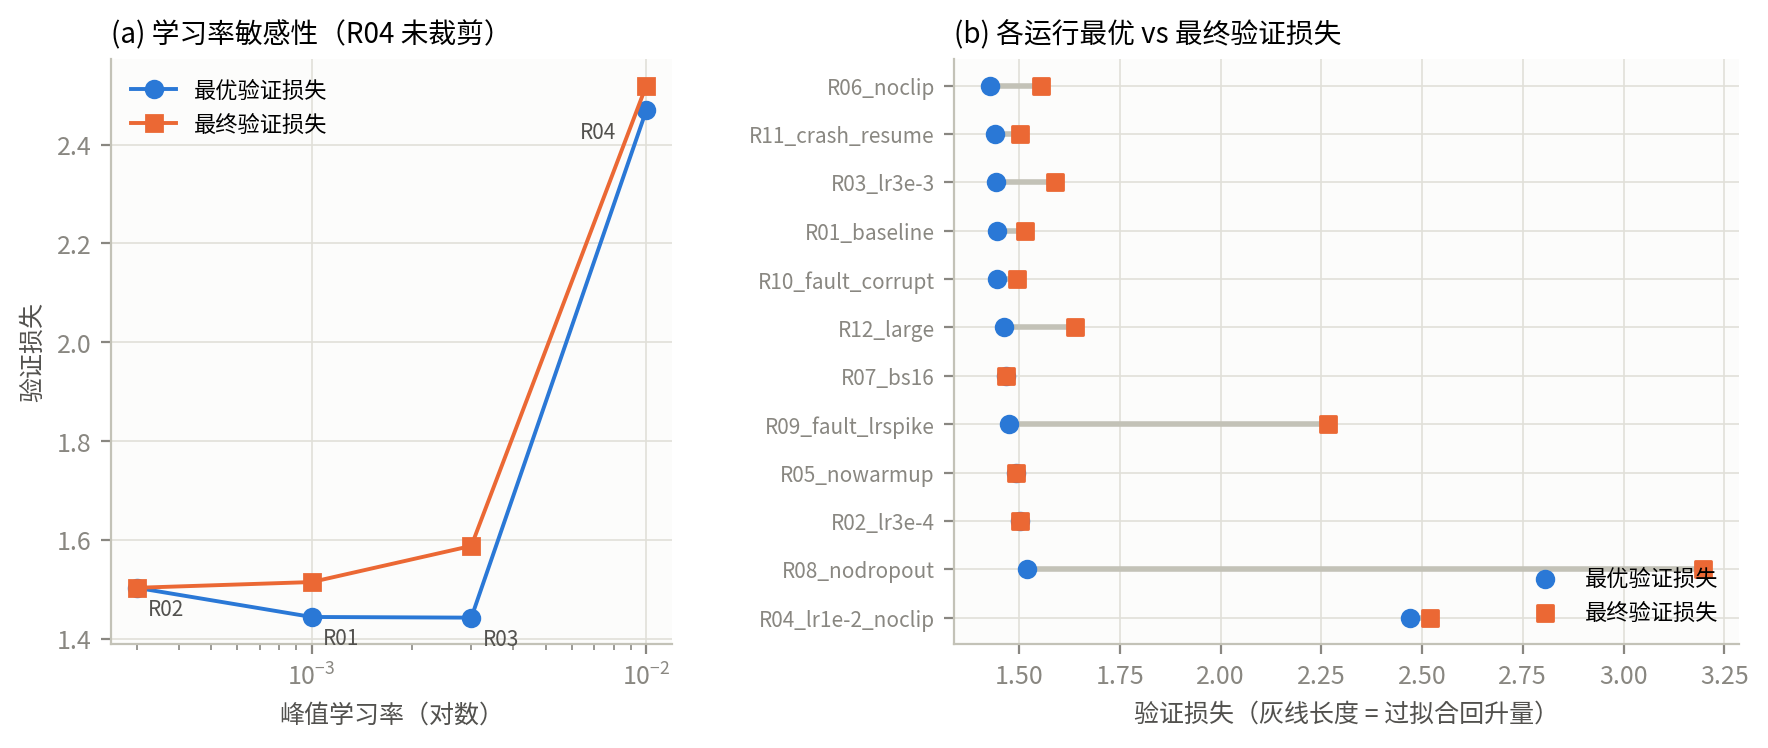
\includegraphics[width=\linewidth]{figures/fig_hparams.png}
\caption{超参数与结果：(a) 学习率敏感性；(b) 各运行最优与最终验证损失（灰线长度即过拟合回升量）}
\end{figure}

结合图 14 与平行坐标视图（图 15），可以总结出以下对训练决策有参考价值的规律：

\begin{enumerate}
\item \textbf{学习率存在明显的“悬崖”}。在 3e-4 到 3e-3 区间，最优验证损失变化不大（1.503$\rightarrow$1.443），但从 3e-3 增加到 1e-2 时，损失跃升到 2.469（R04），性能断崖式下降。曲线在悬崖之前是平坦的，这意味着靠近悬崖的配置“看起来很好”却极其脆弱。实践中应当选择悬崖左侧留有余量的学习率，并用更新比监控与悬崖之间的距离。
\item \textbf{“最优验证”与“最终验证”应分别看待}。图 14(b) 中，高学习率运行（R03、R06）达到最优的速度更快、最优值更低，但随后的过拟合回升也更大（0.145、0.127）；R08（无 dropout）在第 900 步达到 1.518 后一路回升到 3.198，泛化差高达 3.0。总体上，有 5 个运行恰好在第 1300 步达到最优（R11 在第 1400 步），之后开始过拟合，说明在 100 万字符的训练集上，约 21 个 epoch 当量（1300 步 $\times$ 16,384 字符）已经足够，\textbf{早停或保存最优检查点}可以直接带来 0.05–1.68 的验证损失收益。
\item \textbf{扩容不等于变好}。参数量增加 2.35 倍的 R12，最优验证损失（1.4615）反而比基线（1.4439）略差，过拟合回升更大（0.178），同时吞吐减半（45.1 万 vs 88.7 万 tokens/s）、显存增加 1.8 倍。这一结论符合“数据受限时扩大模型收益有限”的缩放规律。
\item \textbf{梯度裁剪是“保险”而非“性能”手段}。R06（不裁剪）的最优值 1.4269 是全场最佳，比裁剪的 R03 低 0.016，但它在第 172 步出现了一次梯度爆炸；R04 则因为不裁剪长期处于梯度爆炸状态。由于每个配置只有一个随机种子，0.016 的差距在噪声范围内，不能据此得出“裁剪有害”的结论。更稳妥的建议是保留裁剪，作为防御极端事件的保险。
\item \textbf{小批量的代价是吞吐而不是精度}。R07（batch=16）的损失波动率是基线的 2.06 倍（0.0485 vs 0.0236），GPU 吞吐只有基线的 68\%，但由于每步处理的样本更少，到第 2500 步时它只看过基线 1/4 的数据，因此仍处于欠拟合阶段，没有出现过拟合（泛化差 0.197）。
\item \textbf{断点续训是安全的}。R11 经历崩溃和续训之后，最优验证损失为 1.4400，与基线的 1.4439 在同一水平（两者随机种子不同），说明检查点中保存的优化器状态和采样器随机状态足以保证续训轨迹的连续性；崩溃带来的真正风险在日志层面（重复与丢失），而这可以由第三章的清洗流程解决。
\end{enumerate}

\begin{figure}[htbp]
\centering
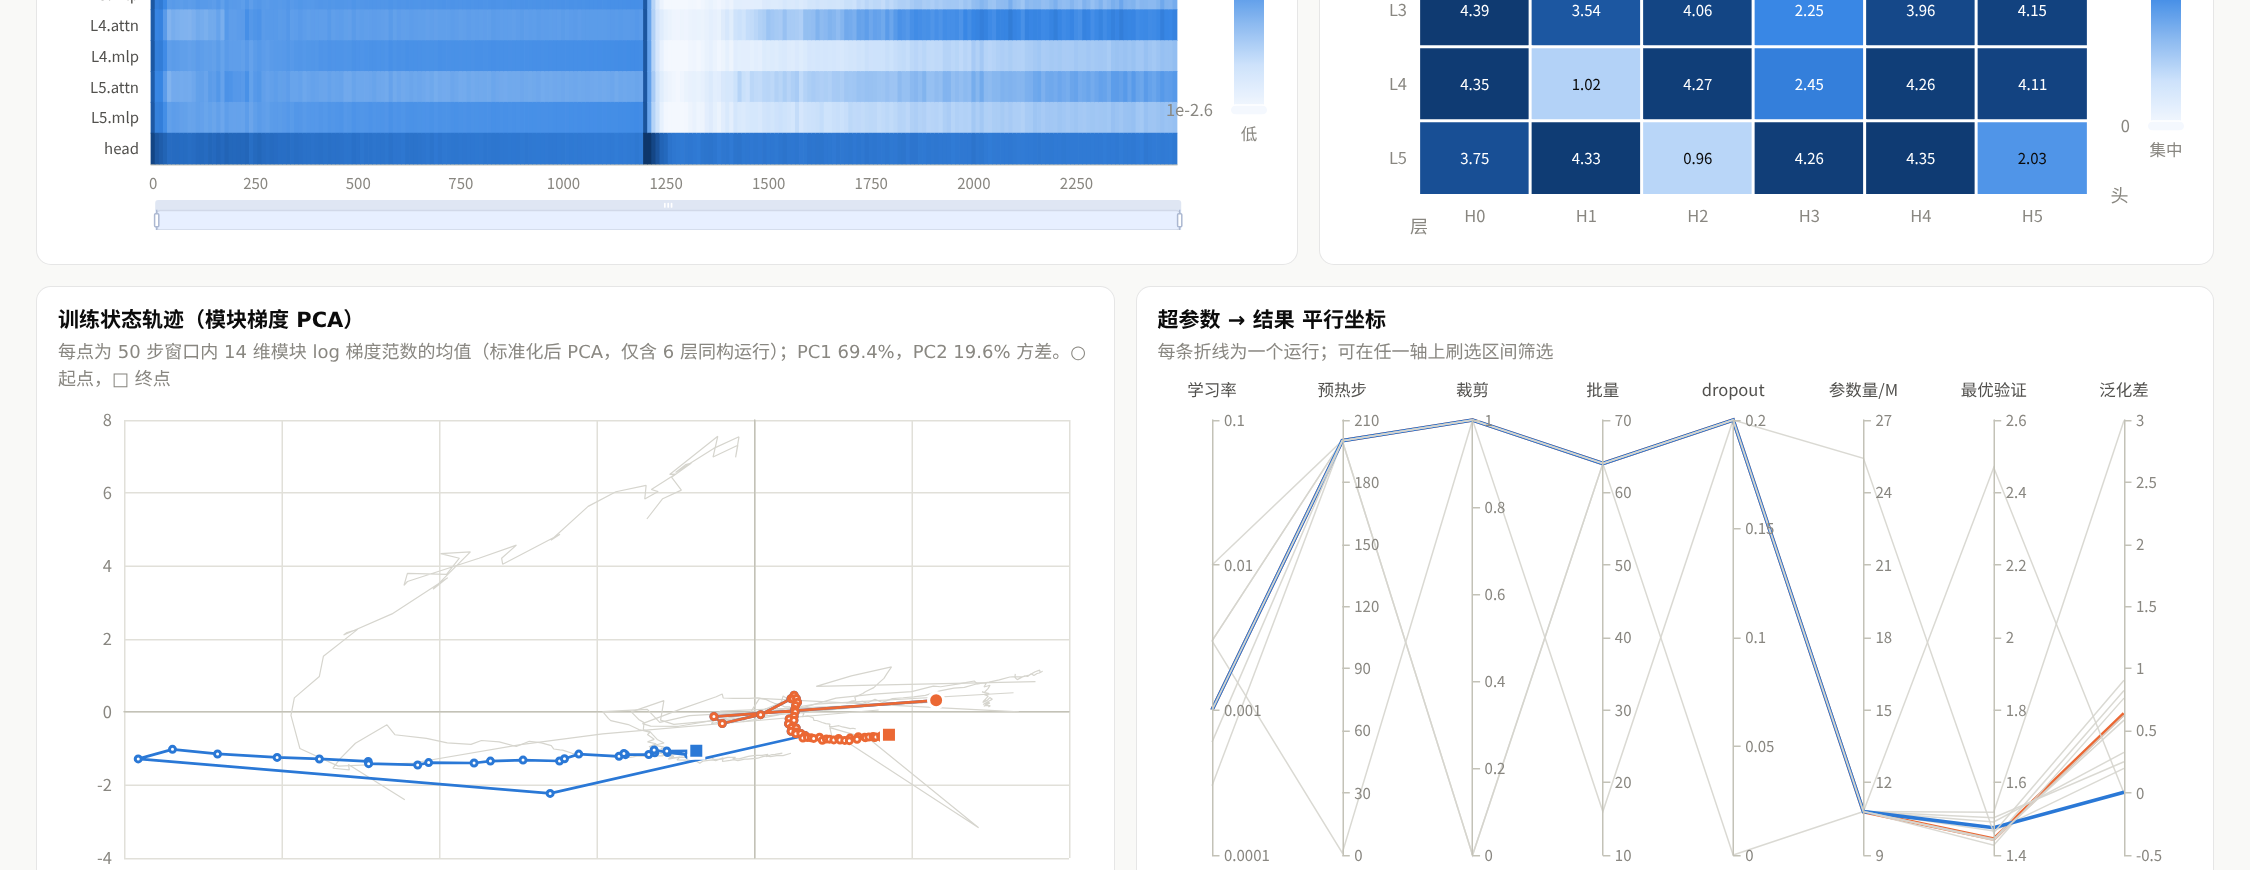
\includegraphics[width=\linewidth]{figures/dash_pca_par.png}
\caption{仪表盘中的 PCA 轨迹视图与超参数平行坐标（焦点 R09 为蓝色，对比 R01 为橙色，其余为灰色背景）}
\end{figure}

\subsection{讨论}

\textbf{可视化与智能体的分工}。在本系统中，智能体负责“把注意力引到正确的地方”，可视化负责“让人信服”。在 R09 与 R10 两个案例中，单看智能体的结论（“学习率异常 99\%”“数据污染 98\%”）用户未必会采信；但当这些结论与联动视图中的证据，如更新比曲线、模块热力图的白色条带、纹丝不动的验证损失，放在一起时，用户可以在几秒钟内自行完成验证。反过来，如果没有智能体，用户需要在 12 个运行 $\times$ 9 个视图中自己寻找异常，效率很低。确定性的知识库加上可回放的执行轨迹，保证了每个结论都可追溯、可复现，这在高成本的训练决策场景中比大模型自由生成的诊断文本更可靠。

\textbf{设计取舍}。focus+context 配色把同时高亮的运行限制在 3 个以内，牺牲了“一眼看到所有运行身份”的能力，换来的是色觉障碍友好和清晰的视觉层次；运行身份可以通过悬停、总览表和小多图（图 5）来补充。拒绝双 y 轴增加了视图数量，但通过联动缩放，多个视图在交互上表现为一个整体。

\section{结论与展望}

\subsection{研究贡献}

本文围绕“大模型训练监控”这一高成本场景，设计并实现了 TrainScope 系统，主要贡献如下：

\begin{enumerate}
\item \textbf{一个真实、可复现的多维训练监控数据集}：12 组 GPT 训练、3 类真实注入故障、61,695 行原始日志，涵盖逐步、逐模块、逐注意力头的指标，并且保留了续训重复、记录丢失、计时污染等真实“脏数据”；
\item \textbf{面向训练日志的清洗与特征工程方法}：续训去重与丢失修复、计时污染识别、稳健 z 分数，以及模块梯度 PCA 轨迹和嵌入 t-SNE 两种降维视角；其中 EDA 直接推动了检测器的两次修正（更新比相对化、注意力塌缩全局化）；
\item \textbf{一个遵循可视化原则的交互式仪表盘}：9 类视图联动缩放、跨视图钻取、注意力动画、focus+context 配色、双主题和 URL 状态分享，并支持自然语言驱动视图操作；
\item \textbf{一个可解释的多智能体诊断工作流}：9 类检测器、取证工具、区分性根因知识库和可回放轨迹。对两个注入故障实现了零延迟检出和正确的根因区分，在健康运行上没有误报；
\item \textbf{若干对训练实践有参考价值的洞察}：学习率尖峰会造成中间层梯度坍缩式的不可逆损伤，而数据污染是可恢复的；缺少预热会引发可恢复的注意力熵塌缩；学习率存在性能悬崖；字符级模型会自发习得大小写对应关系（最近邻命中率 96.2\%）。
\end{enumerate}

\subsection{局限性}

\begin{enumerate}
\item \textbf{规模局限}：实验基于 10.8M/25.4M 参数的字符级模型和单卡训练，没有覆盖真实大模型的分布式训练（多卡通信、流水线气泡、混合精度溢出），一些现象（如损失尖峰的频率与成因）在大规模下可能不同。
\item \textbf{统计效力不足}：每个配置只有一个随机种子，超参数之间的细微差异（如 R06 与 R03 的 0.016）无法给出显著性判断；异常检测评估只有 2 个注入故障，阈值是在同一数据上调整的，存在过拟合风险。
\item \textbf{知识库覆盖有限}：根因规则由人工编写，只覆盖了 9 种根因，对硬件故障、通信死锁、tokenizer 漂移等常见问题还没有建模；置信度来自规则得分的 softmax，并不是经过校准的概率。
\item \textbf{大模型能力未充分评估}：Reporter 的大模型润色是可选功能，本文实验都在离线模板模式下完成，没有定量评估大模型生成内容的忠实度；自然语言交互基于规则式意图识别，覆盖的问句形式有限。
\item \textbf{可用性未经用户研究}：仪表盘的设计依据可视化原则，但没有开展正式的用户实验（任务完成时间、正确率、主观负荷等）。
\end{enumerate}

\subsection{未来研究方向}

\begin{enumerate}
\item \textbf{实时流式监控}：把批处理流程改造为基于 WebSocket 的增量计算，让检测器和视图在训练过程中实时更新，并支持“一键回滚”等闭环操作。
\item \textbf{走向真实规模}：在多机多卡场景下增加通信、显存、数据加载等系统层指标，研究跨层（系统层—优化层—表征层）的联合根因分析。
\item \textbf{学习型检测与知识库}：在更大规模的故障注入语料上训练异常检测与根因分类模型，并用大模型从训练报告和事故复盘文档中自动扩充知识库，同时引入概率校准。
\item \textbf{大模型智能体的忠实度约束}：以本系统的结构化证据作为“工具”，研究大模型智能体在开放式问答中的证据引用和幻觉检测，让自然语言交互从规则式意图识别升级为可组合的视图操作语言。
\item \textbf{开展用户研究}：与有实际训练经验的工程师合作进行对照实验，量化系统在异常定位时间和决策正确率上的提升。
\end{enumerate}

\begin{thebibliography}{99}
\bibitem{r1} ZHANG S, ROLLER S, GOYAL N, et al. OPT: Open pre-trained transformer language models[EB/OL]. arXiv:2205.01068, 2022.
\bibitem{r2} LE SCAO T, FAN A, AKIKI C, et al. BLOOM: A 176B-parameter open-access multilingual language model[EB/OL]. arXiv:2211.05100, 2022.
\bibitem{r3} CHOWDHERY A, NARANG S, DEVLIN J, et al. PaLM: Scaling language modeling with pathways[J]. Journal of Machine Learning Research, 2023, 24(240): 1-113.
\bibitem{r4} ABADI M, BARHAM P, CHEN J, et al. TensorFlow: A system for large-scale machine learning[C]//Proceedings of the 12th USENIX Symposium on Operating Systems Design and Implementation (OSDI). Savannah: USENIX, 2016: 265-283.
\bibitem{r5} BIEWALD L. Experiment tracking with Weights and Biases[CP/OL]. 2020. https://www.wandb.com/.
\bibitem{r6} LIU D, CUI W, JIN K, et al. DeepTracker: Visualizing the training process of convolutional neural networks[J]. ACM Transactions on Intelligent Systems and Technology, 2018, 10(1): 1-25.
\bibitem{r7} HOHMAN F, KAHNG M, PIENTA R, et al. Visual analytics in deep learning: An interrogative survey for the next frontiers[J]. IEEE Transactions on Visualization and Computer Graphics, 2019, 25(8): 2674-2693.
\bibitem{r8} VIG J. A multiscale visualization of attention in the transformer model[C]//Proceedings of the 57th Annual Meeting of the Association for Computational Linguistics: System Demonstrations. Florence: ACL, 2019: 37-42.
\bibitem{r9} DIBIA V. LIDA: A tool for automatic generation of grammar-agnostic visualizations and infographics using large language models[C]//Proceedings of the 61st Annual Meeting of the Association for Computational Linguistics: System Demonstrations. Toronto: ACL, 2023: 113-126.
\bibitem{r10} KARPATHY A. The unreasonable effectiveness of recurrent neural networks[EB/OL]. (2015-05-21). https://karpathy.github.io/2015/05/21/rnn-effectiveness/.
\bibitem{r11} RADFORD A, WU J, CHILD R, et al. Language models are unsupervised multitask learners[R]. OpenAI, 2019.
\bibitem{r12} KARPATHY A. CS231n: Convolutional neural networks for visual recognition—Neural networks part 3: Learning and evaluation[EB/OL]. Stanford University, 2016. https://cs231n.github.io/neural-networks-3/.
\bibitem{r13} VAN DER MAATEN L, HINTON G. Visualizing data using t-SNE[J]. Journal of Machine Learning Research, 2008, 9(86): 2579-2605.
\bibitem{r14} MUNZNER T. Visualization analysis and design[M]. Boca Raton: CRC Press, 2014.
\bibitem{r15} SHNEIDERMAN B. The eyes have it: A task by data type taxonomy for information visualizations[C]//Proceedings of the IEEE Symposium on Visual Languages. Boulder: IEEE, 1996: 336-343.
\bibitem{r16} COHEN J M, KAUR S, LI Y, et al. Gradient descent on neural networks typically occurs at the edge of stability[C]//International Conference on Learning Representations (ICLR). 2021.
\bibitem{r17} ZHAI S, LIKHOMANENKO T, LITTWIN E, et al. Stabilizing transformer training by preventing attention entropy collapse[C]//Proceedings of the 40th International Conference on Machine Learning (ICML). Honolulu: PMLR, 2023: 40770-40803.
\bibitem{r18} XIONG R, YANG Y, HE D, et al. On layer normalization in the transformer architecture[C]//Proceedings of the 37th International Conference on Machine Learning (ICML). PMLR, 2020: 10524-10533.
\bibitem{r19} WORTSMAN M, LIU P J, XIAO L, et al. Small-scale proxies for large-scale transformer training instabilities[C]//International Conference on Learning Representations (ICLR). 2024.
\bibitem{r20} OLSSON C, ELHAGE N, NANDA N, et al. In-context learning and induction heads[EB/OL]. Transformer Circuits Thread, 2022. https://transformer-circuits.pub/2022/in-context-learning-and-induction-heads/.
\bibitem{r21} HONG S, LIN Y, LIU B, et al. Data Interpreter: An LLM agent for data science[EB/OL]. arXiv:2402.18679, 2024.
\bibitem{r22} PASCANU R, MIKOLOV T, BENGIO Y. On the difficulty of training recurrent neural networks[C]//Proceedings of the 30th International Conference on Machine Learning (ICML). Atlanta: PMLR, 2013: 1310-1318.
\end{thebibliography}



\section*{附录 A 复现方式}
\addcontentsline{toc}{section}{附录 A 复现方式}

\noindent 项目地址：\url{https://github.com/RowanDVega/computer-visualization-final}

\begin{Verbatim}[fontsize=\small,frame=single,breaklines,breakanywhere]
git clone git@github.com:RowanDVega/computer-visualization-final.git
cd computer-visualization-final
pip install -r requirements.txt
./run_all.sh                 # 训练 12 组 + 预处理 + 智能体诊断 + 出图 + 仪表盘数据
SKIP_TRAIN=1 ./run_all.sh    # 已有日志时仅重跑分析（< 1 分钟）
# 浏览器打开 web/index.html；URL 参数示例：
#   ?focus=R05_nowarmup&cmp=R02_lr3e-4&zoom=300,1600&theme=dark&q=R09为什么出问题
\end{Verbatim}
